\chapter{Úvod}
\label{uvod}
Nejpopulárnějším způsobem modelování a reprezentace dat pro vykreslování je v~současné době využití trojúhelníkových sítí, ale existují i další přístupy. Jednou z~poměrně populárních alternativ je využití voxelů. I~přes to, že voxelové reprezentace jsou v~real-time grafice v~menšině, lze nalézt spoustu zdrojů a vědeckých článků o~této problematice.

Vzhledem ke změnám možností využití grafické karty, především existenci compute shaderů, je práce s~voxely mnohem jednodušší, než tomu bylo v~dřívějších dobách. Není nutné provádět převod na trojúhelníky a můžeme pracovat s~voxelovými primitivy přímo. Tím se odemyká možnost využití optimalizovaných algoritmů. Tato práce se zabývá zobrazováním voxelových scén za pomocí moderních metod a nástrojů, které jsou vývojářům poskytnuty.

První kapitola si dává za cíl seznámit čtenáře s~řešenou problematikou. Vysvětluje základní principy realistického zobrazování a některé populární metody, jimiž je toho možné dosáhnout. Také popisuje, co jsou voxely, jak se s~nimi dá pracovat v~kontextu rozdělení prostoru a základní metody vykreslování. Dále jsou zde popsány vybrané hierarchické struktury, pomocí kterých lze urychlit průchod voxelovým prostorem. V~poslední řadě obsahuje krátký popis moderního API pro práci s~grafickými kartami: \texttt{Vulkan}.

Kapitola druhá se zabývá návrhem řešení. Je zde popsán způsob reprezentace voxelových dat s~využitím akcelerační struktury a její detaily. Kapitola také vysvětluje navrhovaný způsob vykreslování voxelových scén s~využitím ray casting přístupu.

Následující kapitola se zabývá specifikami implementace. V~prvé radě jsou uvedeny nástroje a knihovny využité v~samotné implementaci. Dále jsou popsány knihovny, které byly v~rámci práce vytvořeny: knihovna obsahující obecné nástroje, knihovna pro usnadnění práce s~\texttt{Vulkan} a \texttt{GLFW}, a knihovna pro vytváření a interkaci s~uživatelským rozhraním. Také je zde popsán algoritmus načítání voxelových scén a jejich převod do tíženého formátu. Poslední sekce krátce popisuje uživatelské rozhraní demonstrační aplikace.

Poslední kapitola se věnuje vyhodnocením dosažených výsledků. V~současné době obsahuje analýzu času převodu scén do octree. Popisuje také paměťovou náročnost transformovaných scén.

\chapter{Teorie}
\label{teorie}
Cílem této kapitoly je seznámit čtenáře s~koncepty nutnými pro pochopení vlastního řešení. Kapitola vysvětluje, co je to voxel a jaká jsou jeho hlavní využití v~počítačové grafice. Také popisuje fotorealistické zobrazování a vykreslování voxelových scén obecně. Jsou zde popsány často používané akcelerační struktury pro vykreslování voxelových modelů.

\section{Realistické zobrazování}
Tato sekce popisuje princip a použití různých technik realistického zobrazování používaného v~současné počítačové grafice. Jsou zde uvedeny pouze relevantní informace související s~tématem a předpokládá se znalost základních termínů.

Realistické zobrazování je podle knihy \cite{gfx_principles_practice} definováno jako tvoření obrazu podle definovaného modelu scény a osvětlení v~ní přítomné. Jednotlivé pixely ve vytvořeném snímku (angl. rendered image) se dají chápat jako množství světla procházejícího podél paprsků ve scéně; to odpovídá integrálu vstupující světelné energie v~bodě, případně v~regionu.

Dle knihy \cite{real_time_render}, základní komponentou zobrazování v~počítačové grafice je zobrazovací řetězec (angl. rendering pipeline). Funkcí zobrazovacího řetězce je vygenerování dvourozměrného snímku daného virtuální kamerou, scénou obsahující vykreslované modely a zdroji světla.

V~článku \cite{render_eq} je představena zobrazovací rovnice. Je to integrální rovnice, jež zobecňuje přenos světelných paprsků ve scéně. Rovnice je ve tvaru

\begin{equation} \label{eq:render}
	\begin{gathered}
		I(x, x') = g(x, x') \Big[\varepsilon(x, x') + \int_S\rho(x, x', x'')I(x', x'')dx''\Big]
	\end{gathered}
\end{equation}

kde $I(x, x')$ je intenzita světla z~bodu $x'$ do bodu $x$, $g(x, x')$ je geometrický term reprezentující zastínění povrchu mezi body $x$ a $x'$, $\varepsilon(x, x')$ značí intenzitu emitujícího světla z~bodu $x'$ do bodu $x$ a $\rho(x, x', x'')$ představuje intenzitu rozptýleného světla z~bodu $x''$ do bodu $x$ přes plochu povrchu $x'$. Integrál je vypočten přes $S = \bigcup S_i$, tedy jako sjednocení všech povrchů, kdy $S_0$ je dostatečně velká hemisféra uzavírající celou scénu.

Jak je dále uvedeno v~článku \cite{render_eq}, rovnice vychází z~fyzikální rovnice radiozity. Popisuje přenos intenzity světla z~jednoho povrchového bodu do jiného jako sumu emitovaného osvětlení a celkové intenzity rozptýleného světla v~bodě $x$ od všech okolních povrchových bodů.

Podobná zobrazovací rovnice byla představena souběžně se dříve zmíněnou rovnicí v~článku \cite{render_eq_2}. Tato rovnice je popsána pomocí vektorů a je v~literatuře používána častěji. Nejznámější formu zobrazovací rovnice popisuje kniha \cite{gfx_principles_practice}:

\begin{equation} \label{eq:render_2}
	\begin{gathered}
		L_{out}(P, \omega_0) = L_e(P, \omega) + \int_{\omega_i\in S^2(p)}L_{in}(P, -\omega_i)f_s(P, \omega_i, \omega_0)(\omega_i \cdot \textbf{n}_P)d\omega_i
	\end{gathered}
\end{equation}
kde $L(P, \omega)$ je příchozí ($L_{in}$) či odchozí ($L_{out}$) světlo v~bodě $P$ ve směru $\omega$, $\textbf{n}_P$ je normála povrchu v~bodě $P$, $\omega_i$ značí příchozí směr světla, $\omega_0$ analogicky odchozí směr světla a $S$ je sjednocení všech povrchů. $L_{out}$ je světlo vyzářené pryč z~bodu $P$ ve směru $\omega_0$ (tedy směrem k~pozorovateli), $L_e$ je emitované světlo, $L_{in}$ je světlo přicházející z~$\omega_i$ a $f_s$ je obousměrná distribuční funkce odrazu světla (BRDF) (světlo odražené z~$\omega_i$ k~$\omega_0$).

Existuje mnoho metod realistického zobrazování, následuje základní popis vybraných.

\subsection{Ray tracing}\label{sec:ray_tracing}
Neboli sledování paprsku. Pravděpodobně nejznámější metoda globálního osvětlení. Kniha \cite{advanced_global} popisuje ray tracing jako algoritmus počítající radianční hodnotu $L_{pixel}$ pro každý pixel ve výsledném obrázku. Tato hodnota je váženou hodnotou osvětlení ve scéně obsaženou v~cestě paprsku:

\begin{equation} \label{eq:rt_1}
	\begin{gathered}
		L_{pixel} = \int_{imageplane}L(p \xrightarrow{} eye)h(p)dp \\= \int_{imageplane}L(x \xrightarrow{} eye)h(p)dp
	\end{gathered}
\end{equation}
kde $p$ je bod na rovině obrázku a $h(p)$ váhová či filtrační funkce, $x$ je viditelný bod od kamery skrze $p$.

\begin{figure}[H]
	\centering
	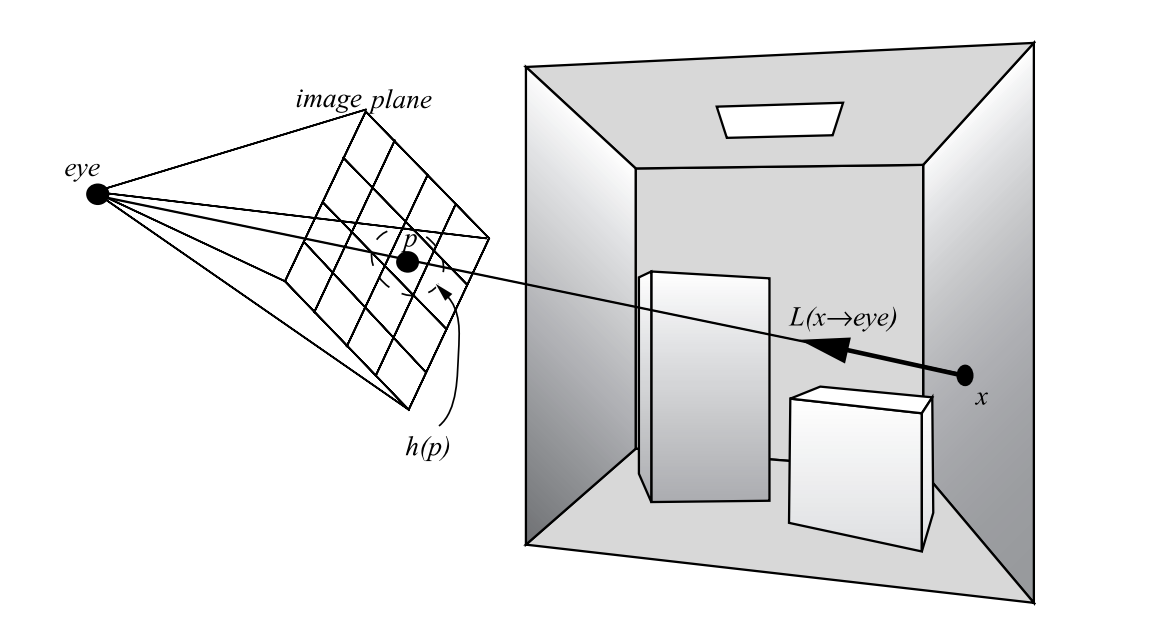
\includegraphics[scale=1]{obrazky-figures/ray_tracing_plane.png}
	\caption{Interakce paprsku se scénou}
	\textbf{Zdroj: \cite{advanced_global}}
	\label{fig:3d_grid}
\end{figure}


Jak název napovídá, ray tracing používá paprsky k~výpočtu barvy výsledného obrázku. Paprsek je polopřímka a je tedy definován počátečním bodem $\Vec{o}$ (origin) a směrem $\Vec{d}$ (direction). Nutnou funkcí pro funkčnost tohoto algoritmu je výpočet průsečíku paprsku s~primitivy, pomocí kterých je scéna vytvořena. Možnosti výpočtu průsečíku paprsku s~voxelem je popsána v~sekci \ref{sec:voxel_intersection}. Jednoduchý ray tracing je popsán v~algoritmu \ref{alg:rt_1}. Takto naivní implementace je samozřejmě velice neefektivní a pro běžně používané scény je nutné použít akcelerační struktury pro urychlení hledání průsečíku \cite{accelerated_rt}. Pro realistické zobrazování jsou krom primárních paprsků generovány i paprsky sekundární. Tyto paprsky jsou použity například pro odrazy, refrakci a stíny.

Ve své standardní formě ray tracing neumožňuje generování měkkých stínů a spousty dalších sekundárních efektů.  Pro dosažení tíženého efektu lze využít například \textbf{Monte carlo ray tracing} (stochaistic ray tracing nebo distributed ray tracing) \cite{distributed_rt}. Namísto jediného paprsku pro výpočet stínů, odrazů a refrakcí je využito paprsků více a výsledky jejich výpočtu jsou následně průměrovány. Metoda umožňuje vytvoření mnoha dalších efektů, jako například hloubka pole, rozmazání pohybu atd.

\begin{center}
	\begin{czechalgorithm}[H] \label{alg:rt_1}
		ray = build\_ray(camera.position, image\_plane)\\
		min\_distance = MAX\\
		hit\_primitive = false\\
		\ForEach{\text{primitive in scene}} {
			(intersected, distance) = intersect(ray, primitive)\\
			\uIf{intersected \And distance < min\_distance}{
				hit\_primitive = primitive\\
				min\_distance = distance\\
			}
		}
		\caption{Ray tracing}
	\end{czechalgorithm}
\end{center}

\subsubsection{Ray marching}
Za zmínku stojí také algoritmus ray marching (sphere tracing). Namísto přímého výpočtu průsečíku se scénou -- jak tomu je u~spousty ray tracing implementací -- postupuje paprsek ve scéně postupně, dokud nedojde k~průsečíku.

\begin{figure}[H]
	\centering
	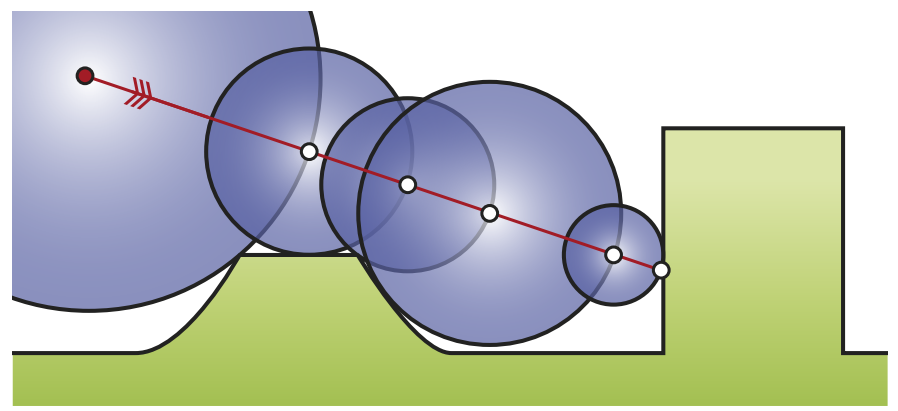
\includegraphics[scale=0.8]{obrazky-figures/ray_marching.png}
	\caption{Ray marching}
	\textbf{Zdroj: \cite{Keinert2014EnhancedST}}
	\label{fig:ray_marching}
\end{figure}

Článek \cite{sphere_tracing} popisuje algoritmus následovně. Podmínkou funkčnosti algoritmu je mít možnost vypočítat z~každého bodu ve scéně vzdálenost k~jejímu povrchu. Pro tento účel lze využít takzvaných signed distance functions (SDF). Pro každý paprsek, kdy generování paprsků probíhá stejně jako u~již zmíněného ray tracing, se iteruje napříč scénou dokud do ní paprsek nenarazí, nepřekoná maximální počet iterací či vykreslovací vzdálenost (algoritmus \ref{alg:ray_marching}).


\begin{center}
	\begin{czechalgorithm}[H] \label{alg:ray_marching}
		i = 0\\
		t = t\_min\\
		\While{t < t\_max \And i < MAX\_ITERATIONS}{\\
			distance\_to\_scene = dist\_func(ray)\\
			\uIf{distance\_to\_scene < \varepsilon}{\\
				\KwRet t\\
			}\\
			t += distance\_to\_scene\\
			i += 1\\
		}\\
		\KwRet t\_max\\
		\caption{Ray marching}
	\end{czechalgorithm}
\end{center}

Pro tento algoritmus existuje značné množství optimalizací \cite{Keinert2014EnhancedST}. Jako je například "over-relaxation", kdy dochází k~záměrně většímu kroku a případnému návratu zpět. Dalším příkladem je namísto sledování paprsku použít kužel, což značně snižuje množství iterací algoritmu.


\subsubsection{Light field probes} \label{sec:light_field_probes}
Metoda globální iluminace využívající ray tracing, byla představena v~publikaci \cite{light_field_probes}. Pracuje na předpokladu, že kontinuální světelné pole scény $\mathcal{L}(x, \omega)$, kde $x \in \mathcal{R}^3$ je bod v~prostoru a $\omega \in S$ je odchozí směr, reprezentuje distribuci osvětlení ve scéně pro všechny body a směry ve scéně. Light field probes reprezentuje tuto distribuci pomocí diskrétního vyobrazení.

Prostor ve scéně je rozdělen pomocí pravidelné mřížky a do každé diskrétní pozice $x'$ je umístěna instance jedné sondy (probe), která mapuje směry $\omega$ kolem $x'$ na: intenzitu osvětlení $\mathcal{L}(x, \omega)$, normály $\vec{n}_x$ v~bodech $x''$ nejblíže bodu $x'$ a hloubkovou mapu mezi $x'$ a body $x''$. K výpočtu těchto hodnot dochází při přípravě scény.

\begin{figure}[H]
	\centering
	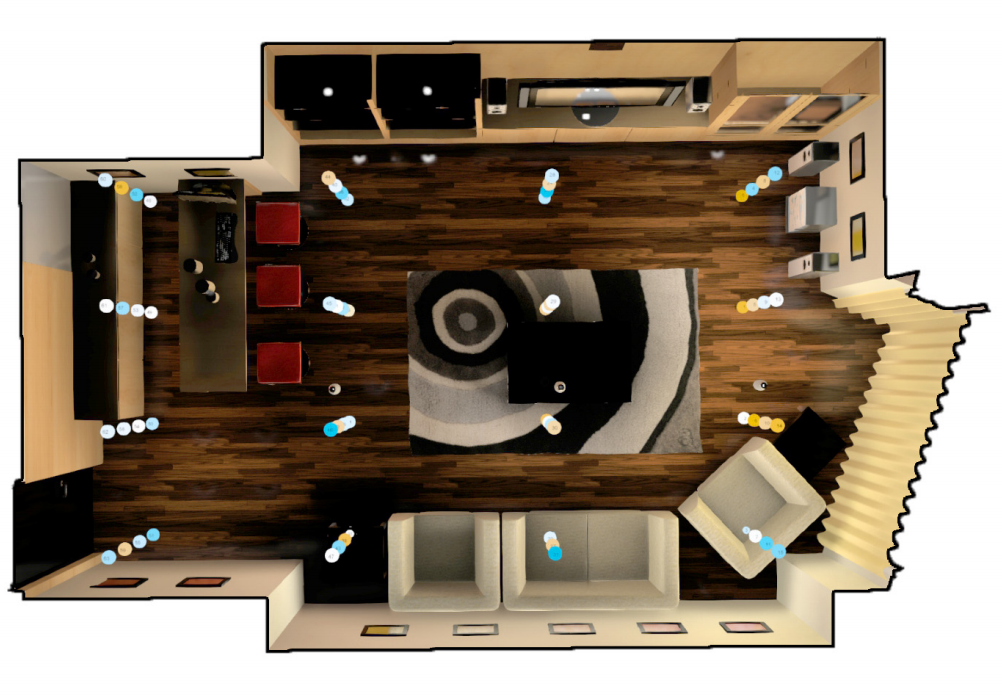
\includegraphics[scale=0.25]{obrazky-figures/light_field_probes.png}
	\caption{Sondy umístěné ve scéně}
	\textbf{Zdroj: \cite{light_field_probes}}
	\label{fig:ray_marching}
\end{figure}

Algoritmus vykreslování postupuje napříč před-připravenými sondami. Při průchodu paprskem dochází k~výběru sondy, trasování uvnitř ní a následně opakuje tento proces napříč scénou, dokud nedojde k~jisté intersekci nebo minutí geometrie scény.

\subsection{Radiozita}
Metody radiozity byly vyvinuty již v~padesátých letech minulého století pro simulaci tepelného přenosu. Později byla popsána varianta pro vykreslování v~článku \cite{radiosity}. Metoda je založena na jednoduchém principu; vzhledem k~tomu, že každý povrch ve scéně může odrážet světlo, se dá tento povrch považovat za zdroj světla. Radiozita povrchu je dána rovnicí:


\begin{equation} \label{eq:voxel_coords}
	\begin{gathered}
		B_i = E_i + \rho_i \sum^N_{j = 1}B_jF_{ij} \text{ pro } i = 1 \text{ do } N
	\end{gathered}
\end{equation}

Kde $B$ je celkové množství energie vyzařované z~povrchu, $E$ je množství energie vyzařované v~povrchu bez vlivu okolí, $\rho$ je faktor reflexivity, $F$ je faktor určující jaká část energie dorazila na povrch a $N$ je počet povrchů ve scéně.

Z~mého průzkumu vyplývá, že je radiozita primárně používána pro předvýpočet globální iluminace v~některých scénách a dále není opakovaně počítána. Důvodem je nejspíše poměrně velká náročnost algoritmu.

\subsection{Materiály}
Pro simulaci interakce světla s~povrchy je nutné mít tyto povrchy popsány určitými parametry. Použité parametry závisí na osvětlovacím modelu a také renderovacímu algoritmu. Publikace \cite{materials} popisuje interakci světla s~povrchem rovnicí:

\begin{equation} \label{eq:surface_photon}
	\begin{gathered}
		(x, y, \theta, \phi, t, \lambda)_{in} \xrightarrow{} (x, y, \theta, \phi, t, \lambda)_{out}
	\end{gathered}
\end{equation}

kde levá strana reprezentuje foton interagující s~povrchem a pravá strana foton vycházející ven, $(x, y)$ je pozice na povrchu, $(\theta, \phi)$ je příchozí/odchozí směr, $t$ je čas interakce a $\lambda$ je vlnová délka. Pro zjednodušení lze z~rovnice odstranit čas, čímž předpokládáme, že se vzhled povrchu s~časem nemění. Při diskretizaci vlnových délek je možné dosáhnout dalšího zjednodušení, čímž dostaneme takzvanou BSSRDF (bidirectional scattering surface distribution function). Dalším zjednodušením může být ignorování podpovrchového rozptylu světla (subsurface scattering), čímž získáme již známé BRDF (bidirectional reflectance distribution function) (rovnice \ref{eq:brdf}).

\begin{equation} \label{eq:brdf}
	\begin{gathered}
		f_r(\vec{c}, \hat{\omega_i} \xrightarrow{} \hat{\omega_0}) = \frac{dL_0(\vec{x}, \hat{\omega_0)}}{dE(\vec{x}, \hat{\omega_i}} \\
		= \frac{dL_0(\vec{x}, \hat{\omega_0)}}{L_i(\vec{x}, \hat{\omega_i)\cos \theta_i d\omega_i}}
	\end{gathered}
\end{equation}

Kde $L_0$ je podíl intenzity světla vycházející z~povrchu na bodu $\vec{x}$ ve směru $\hat{\omega_0}$ a intenzity světla příchozího do bodu $\vec{x}$ ze směru $\hat{\omega_i}$.

Dle knihy \cite{hunter_harold_1987} můžeme materiály dělit do několika základních kategorií podle typu interakce se světlem:

\begin{table}[H]
	\centering
	\begin{tabular}{|l|l|}
		\hline
		materiál              & dominantní distribuce \\ \hline
		průhledný nemetalický & difuzní odraz         \\ \hline
		metalický             & zrcadlový odraz       \\ \hline
		průsvitný             & difuzní přenos        \\ \hline
		průhledný             & běžný přenos          \\ \hline
	\end{tabular}
	\caption{Typy materiálů a jejich interakce se světlem}
\end{table}

\begin{figure}[H]
	\centering
	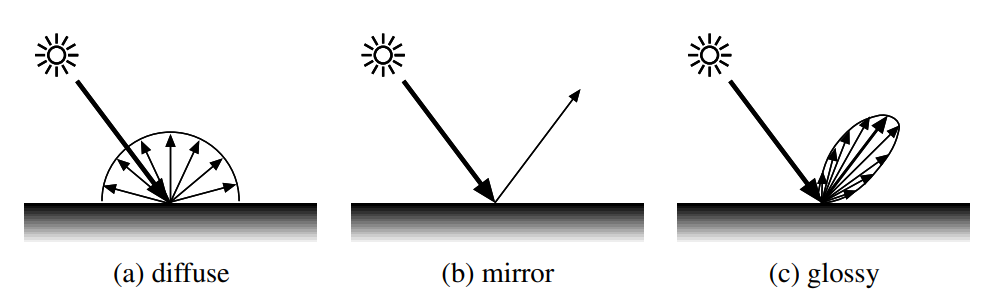
\includegraphics[scale=1]{obrazky-figures/reflection_types.png}
	\caption{Typy odrazu světla (difuzní, zrcadlové, lesklé)}
	\textbf{Zdroj: \cite{materials}}
	\label{fig:3d_grid}
\end{figure}

Dalším podstatným parametrem je tvar povrchu. Tvar povrchu výrazně mění to, jak dochází k~odrazu světla. Vzhledem k~potenciální složitosti této vlastnosti se používají například následující metody:

\begin{itemize}
	\item Mapování normál (normal mapping)
	\item Parallax mapping
\end{itemize}

Příklady některých možných vlastností materiálů:

\begin{itemize}
	\item barva
	\item hrubost
	\item metalické
	\item mapa normál
	\item emisivita
	\item průhlednost
	\item odrazivost
	\item spousta dalších...
\end{itemize}


\subsection{Antialiasing}
Aliasing je nechtěný efekt při zpracování signálu, kdy dochází ke vzniku artefaktů při vzorkování. Při vykreslování se jedná především o~problém při vzorkování textur a artefakty na hranách objektu či přechodu mezi nimi (obrázek \ref{fig:aliasing}). Existuje spousta metod pro odstranění tohoto efektu. Podle \cite{aa_survey} můžeme metody pro antialiasing dělit do následujících kategorií:

\begin{itemize}
	\item Full-Scene Anti-Aliasing (FSAA)
	\item Image Post-Processing Anti-Aliasing (IAA)
	\item Geometric Anti-Aliasing (GAA)
\end{itemize}

Každá z~těchto kategorií má trochu jiný přístup k~problému aliasingu s~různými limitacemi.

\begin{figure}[H]
	\centering
	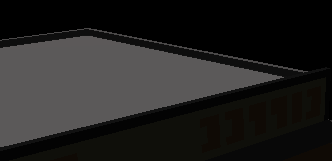
\includegraphics[scale=2]{obrazky-figures/aliasing.png}
	\caption{Aliasing}
	\label{fig:aliasing}
\end{figure}

Příkladem FSAA je \textbf{Super Sampling Anti-Aliasing (SSAA)}, kde je počet pixelů pro renderování navýšen oproti cílové velikosti renderovaného obrázku. Při dokončení jsou přilehlé pixely a jejich barva/hloubka zprůměrovány. Tato metoda dosahuje výborných výsledků, ale je velmi výpočetně náročná. Optimalizovanou alternativou je \textbf{Sampling Ant-Aliasing (MSAA)}. Jedná se o~metodu fungující na stejném principu, ale namísto navýšení rozlišení celého renderovaného snímku dochází k~výběru oblastí, u~kterých je velká pravděpodobnost vzniku aliasingu a super sampling probíhá pouze v~těchto oblastech.

Z~rodiny IAA uveďme\textbf{ Morphological Anti-Aliasing (MLAA)}. Tato metoda si dává za cíl minimalizovat aliasing z~okrajů a siluet. Algoritmus detekuje podezřelé oblasti podle rozdílu sousedních pixelů a používá rozmazání s~okolím. Detekce aliasingu může být i složitější, jako například vyhledávání specifických tvarů.


Vybraný zástupce GAA je \textbf{Geometric PostProcessing AA (GPAA)}. Při renderování obrazu dochází k~ukládání informací o~geometrii scény do separátního bufferu. Podle vzdálenosti sousedních pixelů ve finálním kroku dochází k~rozhodnutí, zda je nutné provádět anti-aliasing. Pokud ano, jsou vypočteny hodnoty okolních pixelů a dochází k~rozmazání.

\begin{figure}[H]
	\centering
	
\includegraphics[scale=3]{obrazky-figures/ssaa_diff.png}
	\caption{Rozdíl kvality obrázku po použití SSAA}
	\label{fig:aliasing}
\end{figure}




\section{Voxel} \label{voxels}
Jak uvádí kniha \cite{gfx_principles_practice}, voxel, neboli \textbf{vo}lume \textbf{el}ement, reprezentuje hodnotu na pravidelné mřížce ve 3D prostoru (obrázek \ref{fig:3d_grid}). Díky tomu, že je prostor rozdělen mřížkou pravidelně, lze voxel definovat pomocí třísložkového vektoru (rovnice \ref{eq:voxel_coords}). Pro účely vykreslování jsou voxelům přiřazovány další vlastnosti, jako například barva nebo materiál.

\begin{equation} \label{eq:voxel_coords}
	\begin{gathered}
		\vec{pozice_{voxel}} \in \mathbb{Z}_3
	\end{gathered}
\end{equation}

\begin{figure}[H]
	\centering
	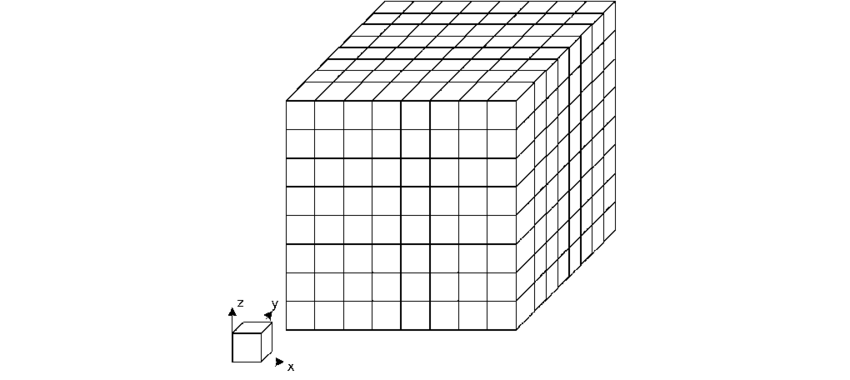
\includegraphics[scale=0.5]{obrazky-figures/3d_grid.png}
	\caption{3D mřížka}
	\textbf{Zdroj: }\cite{3d_grid_image}
	\label{fig:3d_grid}
\end{figure}

Voxely jsou často využívány v~medicíně \cite{medical_vox}, například pro výstupy magnetické resonance (obrázek \ref{fig:mri_vox}).

\begin{figure}[H]
	\centering
	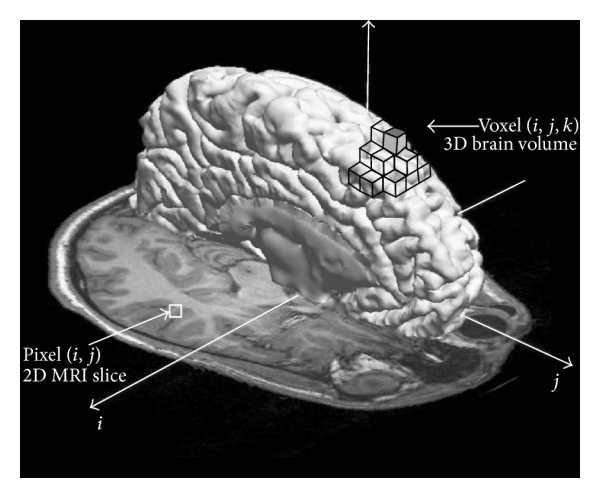
\includegraphics[scale=1]{obrazky-figures/voxel_mri.png}
	\caption{Zobrazení výsledku magnetické resonance pomocí voxelů}
	\textbf{Zdroj: \cite{mri}}
	\label{fig:mri_vox}
\end{figure}

Dalším častým využitím je modelování terénu; voxely přináší možnost reprezentovat převisy, čímž je terén značně realističtější než při aplikaci často používaných výškových map. Pravděpodobně nejznámější software používající voxely pro terén je \texttt{Minecraft} (obrázek \ref{fig:minecraft}). Za zmínku stojí také hra \texttt{Teardown} (2020)\footnote{\url{https://www.teardowngame.com/}}, kde je celý herní svět vytvořen pomocí voxelů a umožňuje téměř neomezenou destrukci.

\begin{figure}[H]
	\centering
	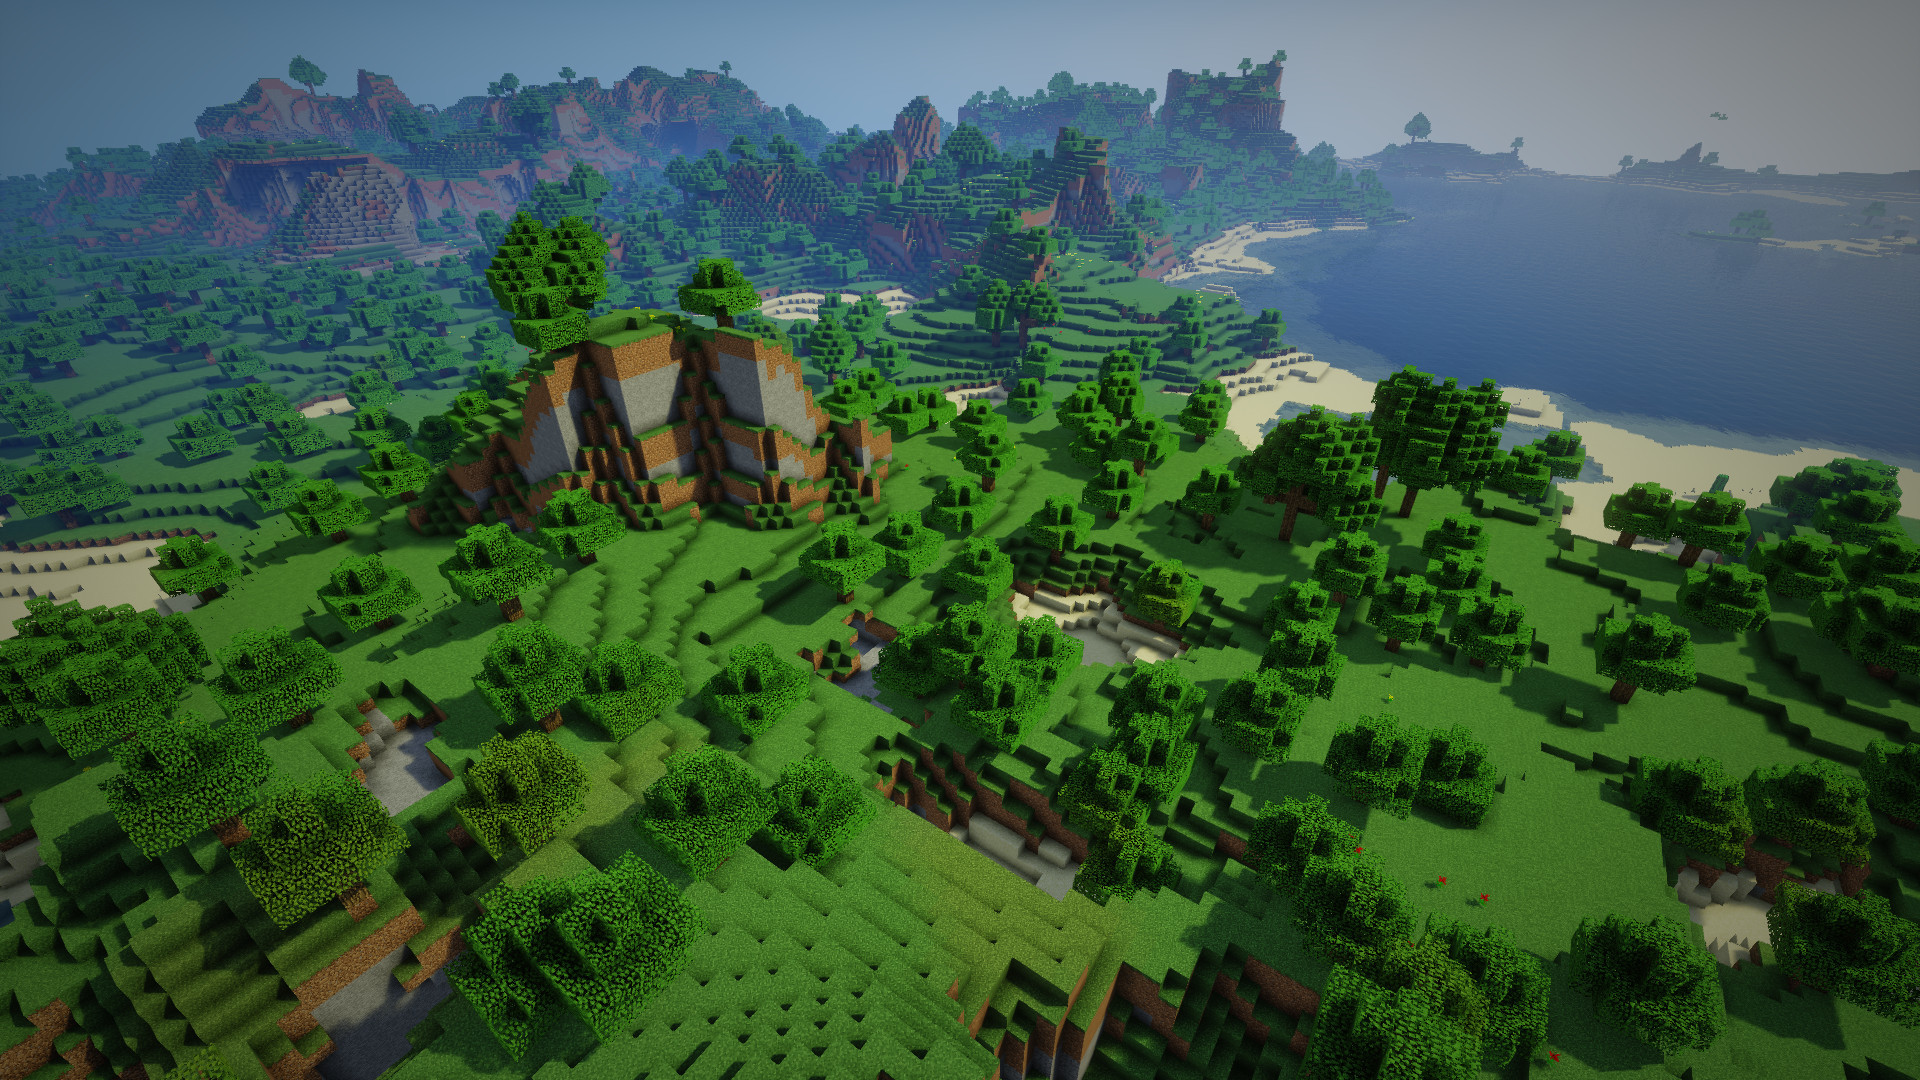
\includegraphics[scale=0.13]{obrazky-figures/minecraft.jpg}
	\caption{Minecraft}
	\textbf{Zdroj: \url{https://forums-cdn.spongepowered.org/uploads/default/original/2X/8/83abd20efc6cf5104c2f8c5459808bcd1addef7a.jpg}}
	\label{fig:minecraft}
\end{figure}

\subsection{Vykreslování voxelových modelů}
Níže jsou popsány základní metody vykreslování voxelových modelů. Jedná se jen o~základní příklady, ve skutečnosti existuje mnohem více metod, než by bylo rozumné zde popisovat.

\subsubsection{Rasterizace}
Pro vykreslování voxelových scén pomocí rasterizace je nutné ji převést na trojúhelníkovou reprezentaci. Toho se dá dosáhnout několika způsoby.

\paragraph{Instanced rendering} je velice primitivní metoda. Pro každý voxel, který je reprezentován přímo svojí pozicí a případně dalšími parametry (barva...), je vykreslena krychle o~předem určené délce hran. Před samotným vykreslováním musí docházet k~odstranění takových voxelů, které nejsou viditelné. Pokud by byl tento krok vynechán, bylo by vykreslování velice náročné. \cite{nousiainen_2019}

\begin{center}
	\begin{czechalgorithm}[H] \label{alg:instanced_cube}
		voxel\_array = cull\_voxels(all\_voxels)\\
		\ForEach{\text{voxel in voxel\_array}} {\\
			render\_cube(voxel.position)\\
		}\\
		\caption{Instancované vykreslování}
	\end{czechalgorithm}
\end{center}

\paragraph{Marching cubes \cite{marching_cubes}} je příkladem algoritmu pro extrakci povrchu z~voxelových dat. Původně představen pro vizualizaci dat v~medicínském odvětví, je současně využíván například pro vizualizaci terénu \cite{nguyen_2008}. Pro každou oblast v~mřížce prostoru je zjištěno, který z~rohů voxelu se nachází uvnitř či vně tělesa. Na základně toho je vypočten tvar a pozice generovaných trojúhelníků. V~některých úpravách algoritmu je možné značně snížit počet vygenerovaných trojúhelníků a snížení redundantnosti dat. Po vygenerování často dochází k~minimalizaci počtu trojúhelníku. Následuje zjednodušená verze algoritmu.

\begin{center}
	\begin{czechalgorithm}[H] \label{alg:marching_cubes}
		\ForEach{voxel in area} {\\
			case = calculate\_case(voxel)\\
			triangles = generate\_triangles(voxel.position, case)\\
			result.add(triangles)\\
		}\\
		\caption{Marching cubes}
	\end{czechalgorithm}
\end{center}

Existují další metody, jako například \textbf{marching tetrahedra}, ale tato práce rasterizačních metod nevyužívá a proto tu nebudou dále zmiňovány.

\subsubsection{Ray casting} \label{sec:voxel_intersection}
Při vykreslování pomocí paprsků lze problém rozdělit na dvě části. První z~nich je výpočet průsečíku s~voxelem a druhým je využití hierarchické struktury pro minimalizaci počtu navštívených voxelů. Hierarchické struktury jsou v~samostatné sekci.

\paragraph{Průsečík paprsku s~voxelem} lze počítat mnoha způsoby. Primitivní přístup k~řešení tohoto problému je počítat průsečík s~každou rovinou, která reprezentuje voxel a následně vybrat ten nejbližší (algoritmus \ref{alg:ray_box_primitive}). Tohle řešení je ale poněkud náročné a využívá podmínky, což může podle článku \cite{gpu_branch} značně zpomalit výpočet.

\begin{center}
	\begin{czechalgorithm}[H] \label{alg:ray_box_primitive}
		corner_1 = voxel.position\\
		corner_2 = voxel.position + voxel\_length\\
		coeffs[0] = (corner_1.x - ray.origin.x) / ray.direction.x\\
		coeffs[1] = (corner_1.y - ray.origin.y) / ray.direction.y\\
		coeffs[2] = (corner_1.z - ray.origin.z) / ray.direction.z\\
		coeffs[3] = (corner_2.x - ray.origin.x) / ray.direction.x\\
		coeffs[4] = (corner_2.y - ray.origin.y) / ray.direction.y\\
		coeffs[5] = (corner_2.z - ray.origin.z) / ray.direction.z\\
		hit = false\\
		distance = \inf\\
		\ForEach{\text{coef in coefs}} {\\
			\uIf {coef >= 0} {\\
				hit = true\\
				hit\_point = ray.origin + ray.direction * coef;\\
				\uIf{is\_in\_box\_bounds(corner_1, hit\_point)}{\\
					distance = coef\\
				}
			}
		}
		\caption{Primitivní výpočet průsečíku s~voxelem}
	\end{czechalgorithm}
\end{center}

Vhodnější alternativou pro výpočet průsečíku paprsku s~voxelem lze najít v~publikaci \cite{efficient_box_intersect}. Tato metoda využívá dlaždic (slabs), kdy je voxel považován za průsečík tří z~nich. Na obrázku \ref{fig:slabs} je vizualizace výpočtu ve 2D - ve 3D je výpočet obdobný. Algoritmus pro 2D je popsán v~rovnici \ref{eq:slabs}.


\begin{equation} \label{eq:slabs}
	\begin{gathered}
		x_{min} = p_x + t_{xmin} d_x\\
		t_{xmin} = \frac{(x_{min} - p_x)}{d_x}\\
		\\
		y_{min} = p_y + t_{ymin} d_y\\
		t_{ymin} = \frac{(y_{min} - p_y)}{d_y}\\
		\\
		t_{xenter} = \min(t_{xmin}, t_{xmax})\\
		t_{xexit} = \max(t_{xmin}, t_{xmax})\\
		\\
		t_{yenter} = \min(t_{ymin}, t_{ymax})\\
		t_{yexit} = \max(t_{ymin}, t_{ymax})\\
		\\
		t_{exter} = \max(t_{xenter}, t_{yenter})\\
		t_{exit} = \min(t_{xexit}, t_{yexit})\\
	\end{gathered}
\end{equation}

\begin{figure}[H]
	\centering
	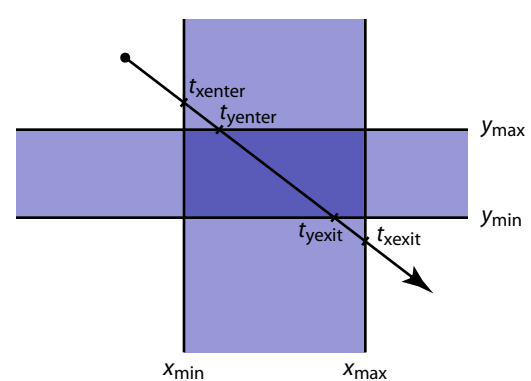
\includegraphics[scale=1.3]{obrazky-figures/slab_intersect.png}
	\caption{Průsečík s~voxelem metodou dlaždic}
	\textbf{Zdroj: \cite{Cunha13}}
	\label{fig:slabs}
\end{figure}


\subsection{Používané formáty} \label{sec:format}
Pro ukládání voxelových scén existuje poměrně velké množství formátů. Bohužel neexistuje žádný standardizovaný formát, i když nějaké pokusy o~to již byly (například VolDat\footnote{\url{http://www.volumesoffun.com/voldat-format/}}). Následuje popis vybraných formátů.

\paragraph{Vox} formát byl vytvořen pro aplikaci MagicaVoxel\footnote{\url{http://ephtracy.github.io/}}, což je modelovací software pro voxelové scény. Jedná se o~binární formát, kde jsou barvy zakódovány pomocí palety. Také podporuje různé typy materiálů, ač s malým množstvím parametrů. Scéna je složena z částí (modelů), které mají maximální velikost 256x256x256 voxelů -- při načítání je tedy nutné se rozhodnout, zda je celý soubor jedním modelem nebo je rozdělen na chunky. Specifikace formátu jsou v~\cite{vox_format}.

\begin{figure}[H]
	\centering
	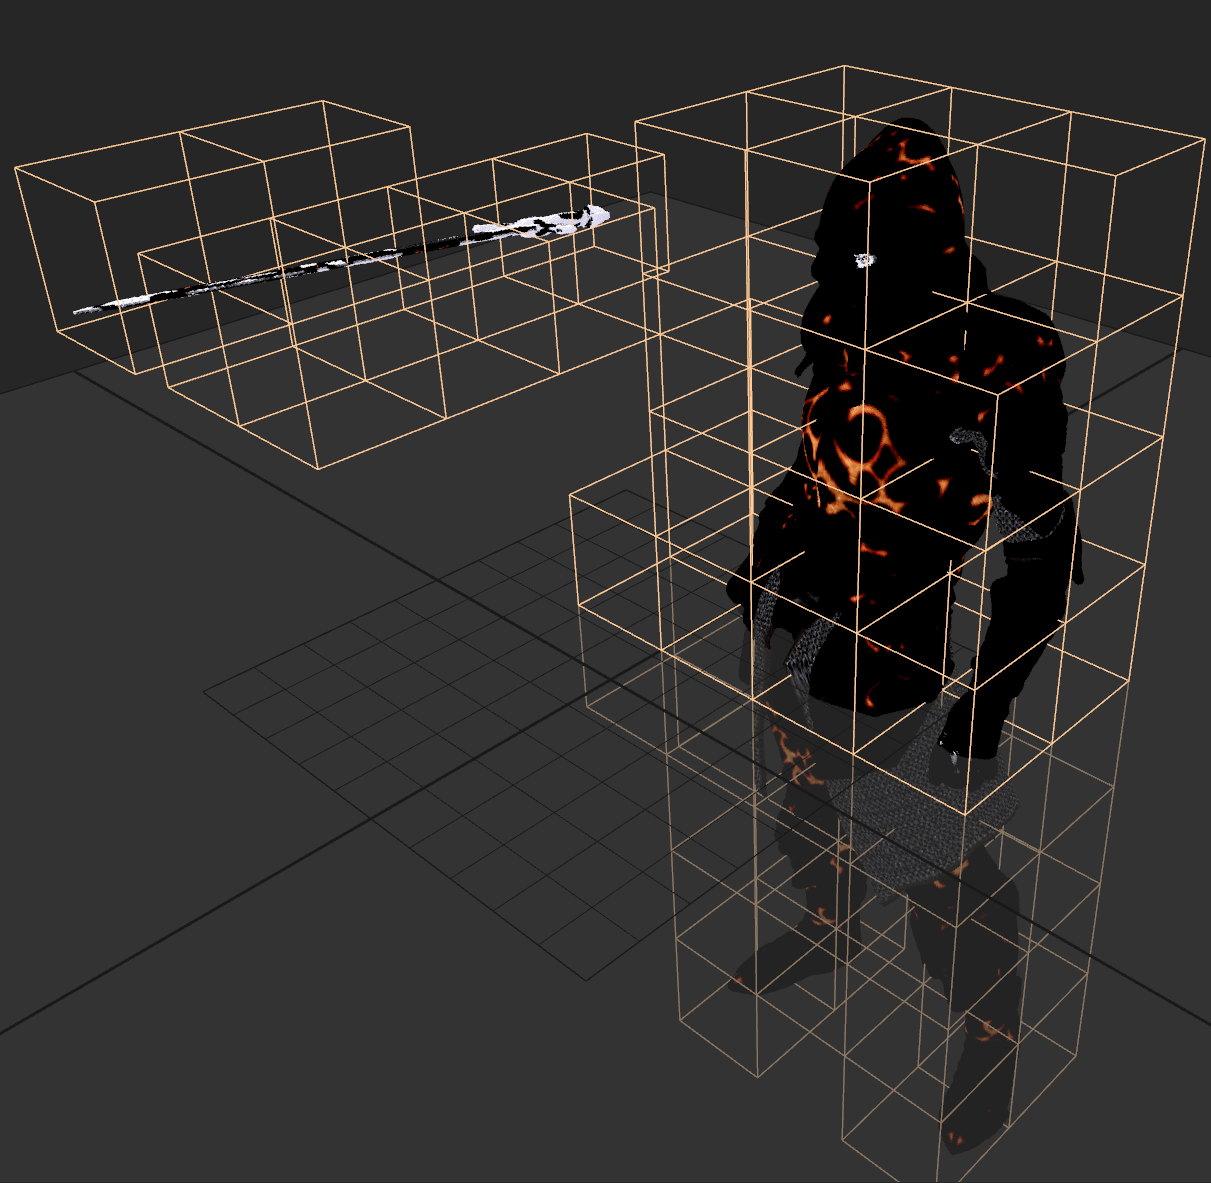
\includegraphics[scale=0.5]{images/magica_voxel_vox.png}
	\caption{Ukázka rozdělení VOX modelu na chunky v programu MagicaVoxel}
	\label{fig:magica_vox}
\end{figure}

\paragraph{SVX} (Simple Voxels) je archivový formát. Archiv obsahuje soubor manifest.xml, který popisuje velikost mřížky, velikost voxelů, paletu materiálů a další metadata. Samotné voxely jsou popsány pomocí obrázků v~jednokanálovém formátu PNG, přičemž každý pixel slouží jako odkaz do palety modelů. Tento formát je používán především pro 3D tisk. Specifikaci formátu najdete na \cite{svx_format_2014}.

Existuje spousta dalších formátů, značné množství pro 3D tisk, ale také pro využití v~medicíně, jak již bylo zmíněno dříve. Dle mého průzkumu je nejčastějším přístupem při volbě formátu pro vykreslovací engine vytvořit formát vlastní.

\paragraph{VolDat} byl vytvořen jako pokus o jistou formu standardizace voxelových formátů. Tento formát byl popsán v \cite{williams_2013}. Scéna je rozdělena na 2D části (průřezy napříč osou Y) a každý tento průřez je uložen v obrázku. Pixely obrázku reprezentují jednotlivé voxely, jejich hodnota vyjadřuje barvu a také odkaz do separátního textového souboru, kde jsou uloženy doplňující data, jako například informace o materiálech. 


\section{Hierarchické struktury}
Jak již bylo zmíněno, pro efektivní práci s~velkým množstvím voxelů je potřeba využít akceleračních struktur. V~této sekci najdete popis některých struktur, které se dají pro voxely použít.

\subsection{Mřížka}
Mřížka, nebo také grid, je poměrně jednoduchá struktura pro dělbu prostoru. Na nejnižší úrovni může mřížka odpovídat té, pomocí které dělí prostor samotné voxely. V~takovém případě by však nedošlo k~žádnému zrychlení. Pro akceleraci je prostor obsahující voxely rozdělen do několika částí (tzv. chunks). V~těchto oblastech jsou voxely sdružovány a při hledání požadované položky můžeme nejdřív vybrat správný chunk a pak teprve vyhledávat v~omezené množině voxelů. Samotná struktura má minimální paměťové nároky, ale nepřináší velké zrychlení, alespoň ve srovnání s~ostatními metodami. Jednoduchá trojrozměrná mřížka je na obrázku \ref{fig:3d_grid}.

\subsection{Hierarchie obalových těles} \label{sec:BVH}
Obalové těleso (bounding volume) je jednoduchý geometrický objekt, který obaluje jeden či více objektů s větší komplexitou \cite{ericson_2005}. Důležitým faktorem pro vhodnost tělesa k využití v hierarchii obalových těles (bounding volume hierarchies) pro ray tracing je náročnost výpočtu průsečíku s tělesem. Jako příklad můžeme uvést kouli (rovnice \ref{eq:sphere_ray_intersection}), osově zarovnaný obdelník (axis aligned box) nebo konvexní obálku. 

\begin{equation} \label{eq:sphere_ray_intersection}
	\begin{gathered}
	    R(t) = \textbf{o} + t\textbf{d}  \\
	    
	    (P + t\textbf{d} - C) (P + t\textbf{d} - C) = r^2
	    
	\end{gathered}
\end{equation}

\begin{eqexpl}[60mm]
\item{$R$} paprsek
\item{$\textbf{o}$} počátek paprsku
\item{$t$} vzdálenost průsečíku
\item{$\textbf{d}$} směr paprsku
\item{$C$} střed koule
\item{$r$} poloměr koule
\end{eqexpl}

Samotná hierarchie těchto těles je tvořena jako stromová struktura, kdy každý nelistový uzel obsahuje zpravidla 2 potomky. Obalové těleso reprezentující nelistové uzly je vytvořeno tak, aby ohraničovalo pouze prostor nutný k obsažení jeho potomků.

\begin{figure}[H]
	\centering
	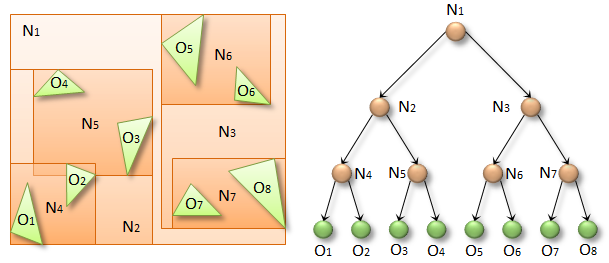
\includegraphics[scale=0.5]{images/fig03-bvh.png}
	\caption{2D hierarchie obalových těles}
	\textbf{Zdroj: \url{https://developer.nvidia.com/blog/thinking-parallel-part-ii-tree-traversal-gpu/}}
	\label{fig:slabs}
\end{figure}

Díky snadnosti výpočtu průsečíků a možnosti netestovat průsečíky s nižšími úrovněmi stromu -- a tím i komplexními objekty -- může dojít k výraznému zrychlení výpočtu průsečíku se scénou. Algoritmus \ref{alg:bvh_traverse_naive} popisuje jednoduchý průchod binárním stromem za pomocí zásobníku.

\begin{center}
	\begin{czechalgorithm}[H] \label{alg:bvh_traverse_naive}
		current\_node = root\\
		stack = empty()\\
		exit = false\\
		\While{\text{!exit}} {\\
			\eIf{isInternalNode(current\_node)}{
			    \uIf{intersectNode(current\_node)}{
			        pushStack(stack, current\_node.first\_child)\\
			        current\_node = current\_node.second\_child\\
			    }
			}{
			    intersectLeaf(current\_node)\\
			    (current\_node, exit) = popStack(stack)\\
			}
		}\\
		\caption{Průchod BVH stromem pro ray tracing \cite{Vaidyanathan2019WideBT}}
	\end{czechalgorithm}
\end{center}



\subsection{Octree} \label{octree}
Octree, poprvé představen v~knize \cite{rensselaer1980octree}, je popsán jako hierarchický N-dimenzionální binární strom, jenž reprezentuje N-dimenzionální objekt. Pro naše účely podstatná pouze jeho 3D varianta. Každý uzel stromu obsahuje 8 potomků na další úrovni. Tyto uzly reprezentují oblast v~prostoru. Pokud uzel kompletně popisuje oblast, kterou reprezentuje, jedná se o~list nebo koncový uzel, v~opačném případě musí obsahovat 8 potomků pro podoblasti. Při hledání objektů v~prostoru tedy můžeme procházet pouze velmi omezenými oblastmi a neplýtvat výpočetní výkon.

\begin{figure}[H]
	\centering
	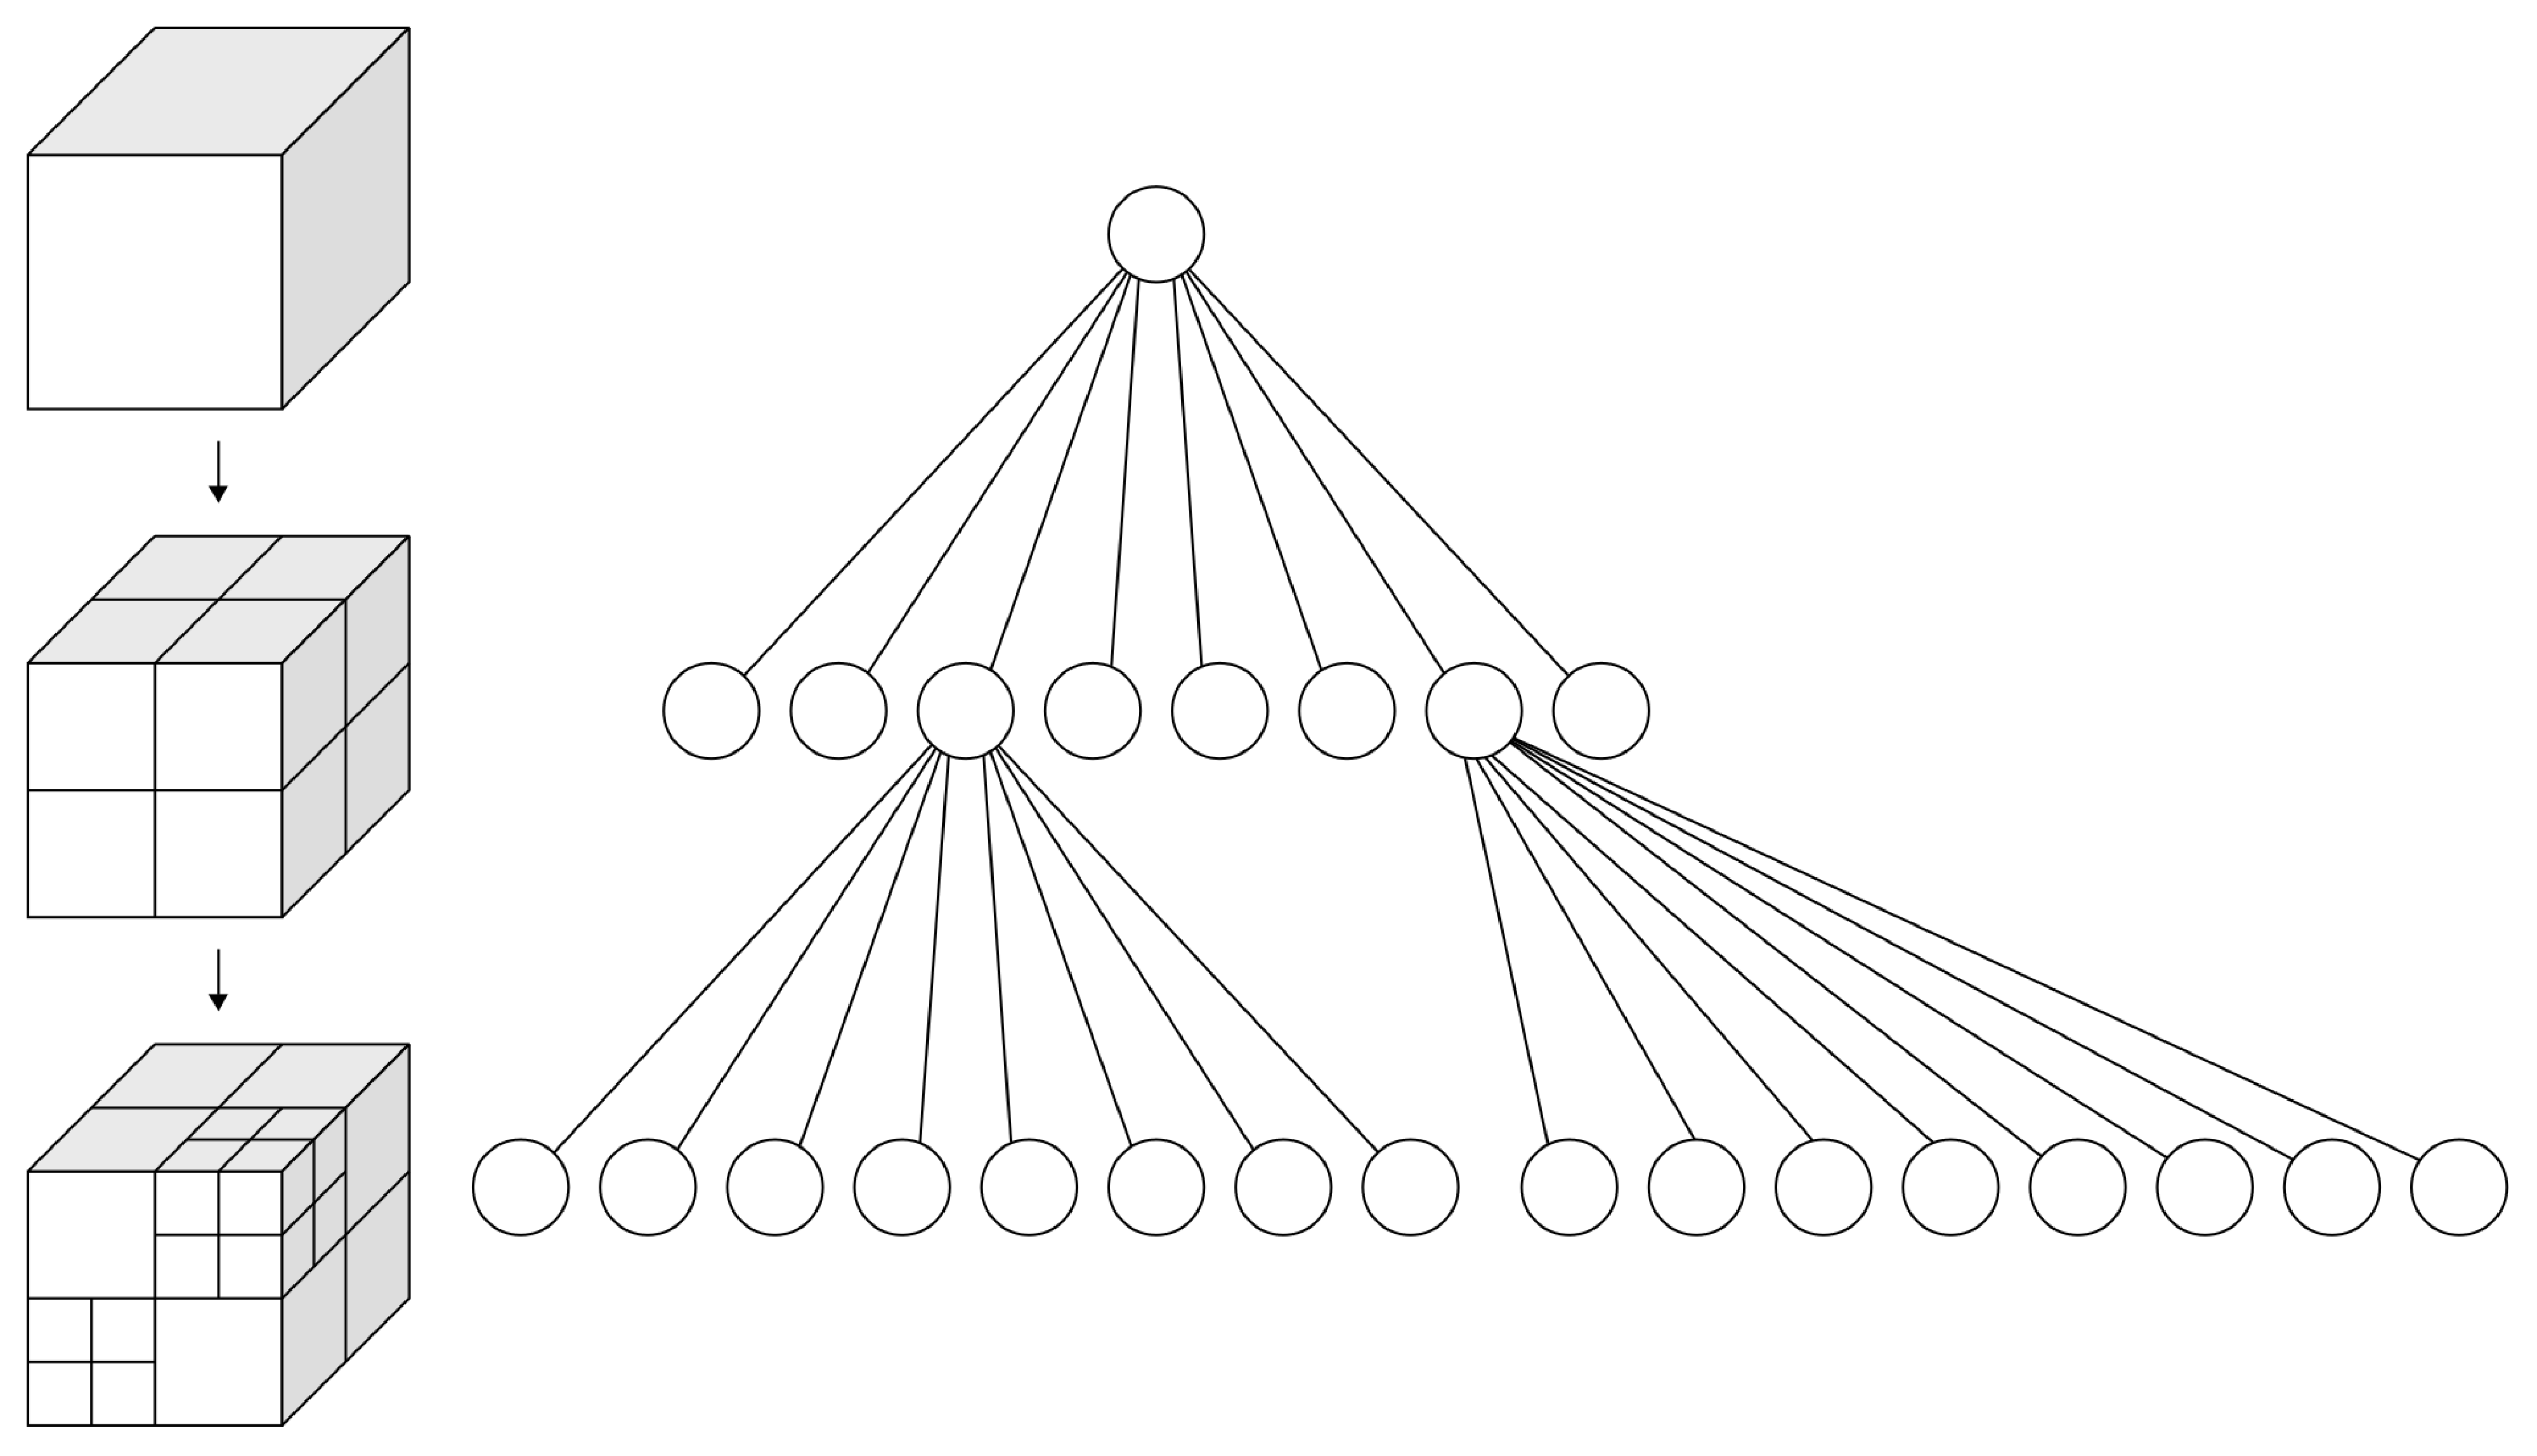
\includegraphics[scale=0.1]{obrazky-figures/Octree2.pdf}
	\caption{Octree}
	\textbf{Zdroj: \url{https://en.wikipedia.org/wiki/Octree}}
	\label{fig:slabs}
\end{figure}


\subsubsection{Sparse voxel octree}\label{svo_alg}
Renderovací metoda využívající ray casting/tracing pro vizualizaci voxelových scén. Důležitou částí generování octree pro tento algoritmus je minimalizace uzlů, které nejsou viditelné, či spojení stejných uzlů do jednoho bloku na vyšší úrovni \cite{Laine2011EfficientSV}. Výhodou je velmi snadná aplikace level of detail napříč stromem. Podle velikosti pixelu je možné zastavit průchod stromem před dosažením nejnižší úrovně a vypočítat výslednou barvu z~uzlu na vyšší úrovni. Algoritmus \ref{alg:svo} popisuje jednoduchou verzi algoritmu.

\begin{center}
	\begin{czechalgorithm}[H] \label{alg:svo}
		voxel = tree.get\_root()\\
		\While{not terminated}{\\
			(hit, t) = intersect\_cube(ray, voxel)\\
			\uIf{hit}{\\
				\uIf{is\_voxel\_small(voxel, pixel\_size) || is\_voxel\_leaf(voxel)}{\\
					\KwRet t\\
				}\\
				stack.push(voxel)\\
				voxel = select\_child(voxel)\\
				continue
			} \uElse {\\
				voxel = stack.pop()
			}\\
		}\\
		\KwRet false
		\caption{Sparse voxel octree ray casting}
	\end{czechalgorithm}
\end{center}

\section{Vulkan API}
Vulkan je API pro 3D grafiku a výpočty pomocí GPU \cite{vulkan_web}. Cílem Vulkan je poskytnout uživateli možnost vyvíjet vysoce výkonné grafické aplikace. V~porovnání s~OpenGL či podobnými staršími API přináší výrazně vyšší výkon, ovšem práce s~ním je poněkud časově náročnější, jelikož Vulkan pracuje na výrazně nižší úrovni, než jeho předchůdci. Byl také navržen s~předpokladem, že bude používán z~více vláken. Některé výhody Vulkan oproti předchozím grafickým API:

\begin{itemize}
	\item Jednotné API jak pro mobilní zařízení, tak pro PC.
	\item Dostupnost na velkém množství operačních systému (podobně jako OpenGL).
	\item Nízký overhead driverů.
	\item Pro shadery používá binární formát SPIR-V\footnote{\url{https://www.khronos.org/opengl/wiki/SPIR-V}}, díky čemuž můžou vývojáři distribuovat pouze binární formu shaderů.
	\item Sjednocení grafického (graphics pipeline) a výpočetního (compute shaders) API.
	\item Ray tracing pomocí rozšíření (tuto funkci podporuje i DirectX12).
\end{itemize}

Současnou verzí API je Vulkan 1.2.184\cite{vulkanspec}.

\chapter{Návrh řešení}
\label{navrh}
V~této kapitole je popsán návrh aplikace pro realistické zobrazování voxelových scén. Kapitola je rozdělena na část popisu reprezentace voxelových dat a dále jejich vykreslování pomocí sparse voxel octree algoritmu.

\section{Reprezentace voxelových dat}\label{sec:voxel_representation}
Jak bylo popsáno v~sekci \ref{voxels}, voxely jsou reprezentovány svou pozicí a jejich materiální vlastnosti různými parametry. Logickým krokem je rozdělení těchto dvou věcí. V~některých strukturách můžeme kódovat implicitně a nemusíme tedy plýtvat paměťovým prostorem.

Pro implicitní zakódování pozice lze využít octree (sekce \ref{octree}). Nejnižší úroveň stromu reprezentuje samotné voxely a jediným nutným parametrem je počáteční pozice stromu a velikost prostoru, který obaluje. Samotný strom by mohl být vytvořen se statickým rozestupem rodičů a potomků, kde by se výpočet indexu následníka mohl řídit rovnicí:

\begin{equation} \label{eq:simple_octree_index}
	\begin{gathered}
		I_{child_j} = (i * 8) + j
	\end{gathered}
\end{equation}

kde $I_{child_j}$ je index $j$-tého potomka, $i$ je index současného uzlu. Při použití tohoto rozložení by ovšem musela být celá oblast uvnitř octree rozdělena na nejmenší bloky a docházelo by k~obrovskému plýtvání paměti.

Úsporný způsob pro reprezentaci octree byl představen v~\cite{Laine2011EfficientSV}. Metoda kóduje informace o~uzlu bitově na data o~velikosti 4 bytů. Vizualizace je na obrázku \ref{fig:octree_child}. Každý nelistový uzel je reprezentován svými daty, listové uzly jsou implicitně kódovány pomocí masek. \texttt{Child pointer} určuje pozici potomků uzlu pro daný uzel. Je uložen jako rozdíl od pozice současného uzlu, čímž si jej můžeme dovolit reprezentovat menším rozsahem. Přepínač \texttt{far} určuje, zda \texttt{child pointer} odkazuje na pozice potomků, či na 32 bitový ukazatel na ně - při velkých stromech nemusí být 15 bitů dostačující. Tento pointer je uložen v~oddělené části bufferu. \texttt{Valid mask} je bitová maska o~velikosti 8 bitů, pokud je hodnota nastavena na 1, pak je ve stromu potomek na tomto indexu reprezentován. \texttt{Leaf mask} odpovídá funkci \texttt{valid mask}, dává nám ovšem vědět, jestli je potomek na indexu terminálním uzlem. Pokud je tedy nastavena na 1, tak je vyhledávání ve stromu na této úrovni ukončeno.

\begin{figure}[H]
	\centering
	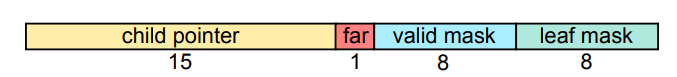
\includegraphics[scale=1.3]{obrazky-figures/octree_child_data.png}
	\caption{Položka reprezentující uzel octree}
	\textbf{Zdroj: \cite{Laine2011EfficientSV}}
	\label{fig:octree_child}
\end{figure}

Samozřejmě krom informací o~obsazenosti prostoru je nutné ukládat i informace o~materiálu. První možností by bylo rozšířit záznamy ve stromu o~tato data, ale s~velkým množstvím parametrů by velikost stromu rapidně narostla. Proto by bylo vhodnější tato data ukládat separátně. Tyto informace také nejsou relevantní při procházení stromu a pokud by byla uložena ve struktuře, došlo by ke zhoršení prostorové lokality paměti. Vhodným řešením je za oblastí stromu vytvořit oblast s~ekvivalentní strukturou, kde jsou uloženy odkazy na materiálová data. Výpočet offsetu do struktury je triviální, jelikož je pozice dat na stejném indexu jako je index uzlu. Nalezené položky slouží k~vyhledávání specifického záznamu v~separátním bufferu. Výhodou tohoto přístupu je možnost snadno ukládat samostatné materiály pro vyšší úrovně stromu, což může být použito pro aplikaci level of detail.

\paragraph{Ukládání voxelových dat}. Pro načítání modelů je využit formát VOX, který byl popsán v sekci \ref{sec:format}. Při načítání je ovšem nutné data transformovat do formátu octree popsaného výše, což může způsobit výrazné zpomalení aplikace. Namísto opakované transformace by bylo tedy vhodné data ukládat tak, aby docházelo pouze k načtení, tím by došlo k výraznému zrychlení. Vzhledem k tomu, že je pro nás důležitá spíše rychlost a ne využití místa na disku je dostačující serializovat strukturu popsanou výše přímo do binárního souboru. Zpravidla dojde k malému zvětšení oproti VOX, ale doba načítání se zkrátí na zlomek času.

\section{Vykreslování}\label{sec:rendering}
V této sekci jsou popsány metody využité pro vykreslování scény v této práci. Je zde popsán ray marching pomocí sparse voxel octrees, light field probes a jejich modifikace pro nepřímé osvětlení.

\subsection{Sparse voxel octree}
Pro rendering voxelové scény existuje několik možností, vhodným kandidátem je přístup sparse voxel octree (sekce \ref{svo_alg}). Při vržení paprsku dochází k~procházení stromu a vcházení pouze do podoblastí, které mohou obsahovat vyhledávaný voxel. Algoritmus je velice úsporný oproti primitivním metodám. Tato metoda je popsána v \cite{Laine2011EfficientSV}.

\begin{figure}[H]
	\centering
	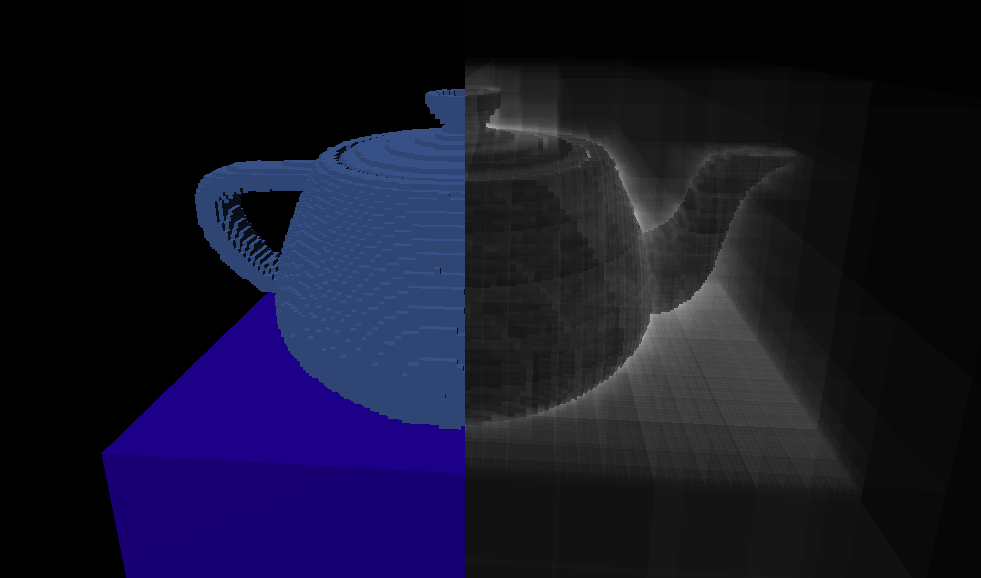
\includegraphics[scale=1]{obrazky-figures/color_iter_svo.png}
	\caption{Render voxelizované "Utah teapot", vlevo barevný výstup, vpravo počet iterací }
	\label{fig:octree_child}
\end{figure}

Vzhledem ke způsobu uložení dat, který byl představen v~minulé sekci, je v~rámci algoritmu nutné dopočítávat množství indexů uzlů na základě masek (\texttt{valid mask} a \texttt{leaf mask}). Jedná se ale zpravidla pouze o~operace sčítání či odčítání a nejsou tedy příliš výpočetně náročné.

Pro výpočet průsečíku s~voxelem je vhodné využít optimálnější metody popsané v~sekci \ref{sec:voxel_intersection}. Důležitou součástí pro stínování je také získání normály povrchu. Vzhledem k~tomu, že mám v~úmyslu zachovat "krychlovitý" tvar voxelů, je nalezení normály při využití slab metody pro nalezení průsečíku poměrně triviální.

\begin{figure}[H]
	\centering
	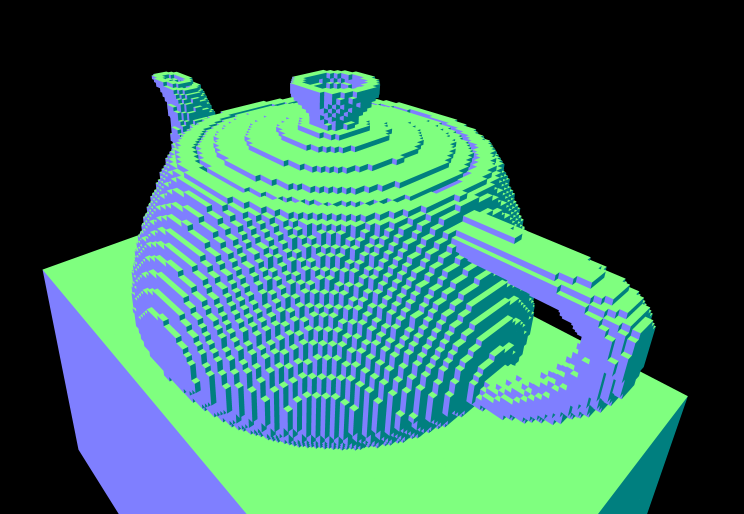
\includegraphics[scale=1]{obrazky-figures/normals_teapot.png}
	\caption{Render voxelizované "Utah teapot", vizualizace normál }
	\label{fig:octree_child}
\end{figure}

Pro usnadnění práce s modely a úsporu výpočetního výkonu při jejich transformaci má každý model svoji vlastní octree strukturu. Nutnost otestovat průsečíky se všemi těmito modely by byla velice náročná a proto je vhodné použít další akcelerační strukturu k urychlení nalezení průsečíku. Zvolil jsem hierarchii obalových těles (sekce \ref{sec:BVH}) s využitím osově zárovnaných obdelníku. Každý listový uzel této hierarchie tedy obsahuje jeden octree, který definuje voxely modelu. 

\begin{figure}[H]
	\centering
	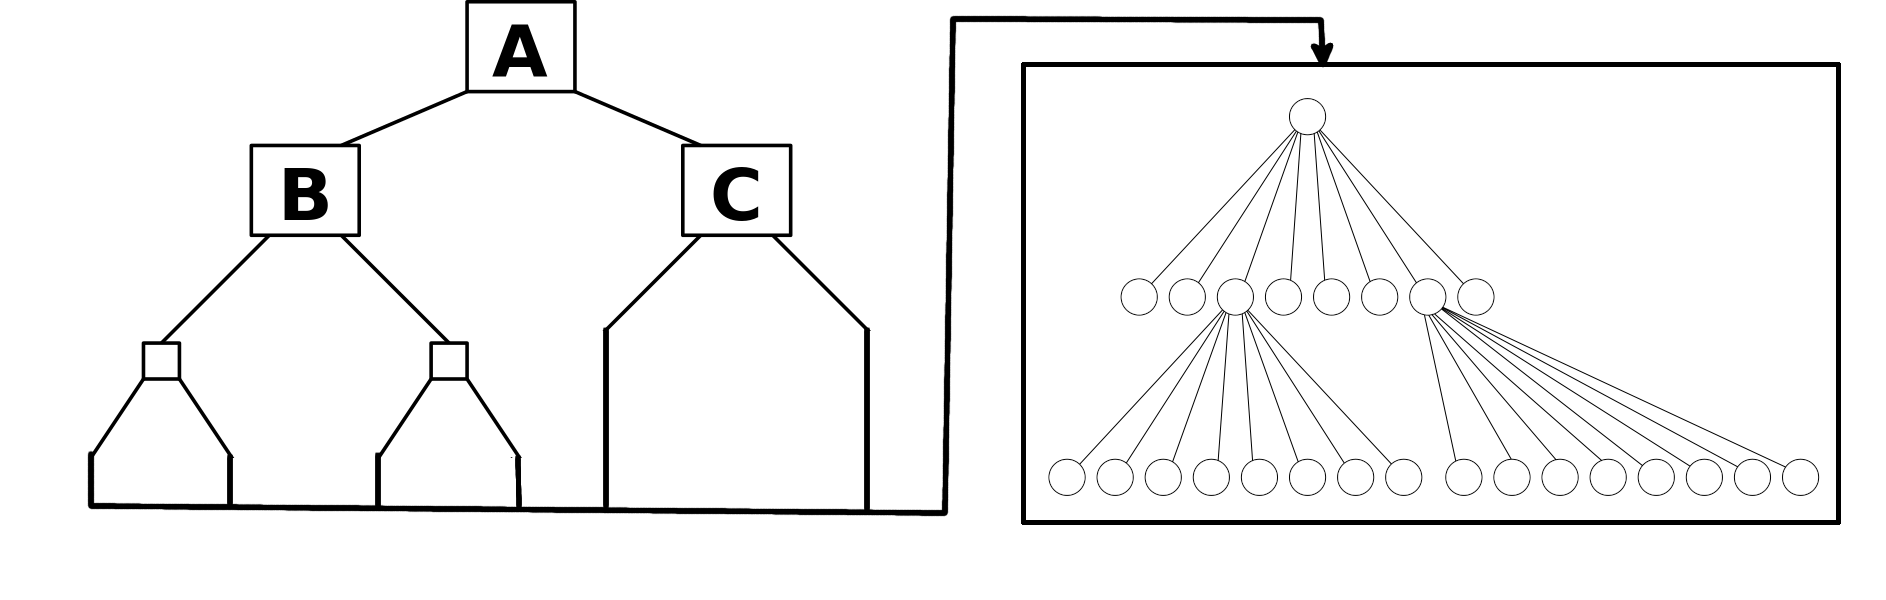
\includegraphics[scale=1]{images/bvh_octree.png}
	\caption{Reprezentace scény - levá část reprezentuje hierarchii obalových těles, obsahující v listech octree (vpravo)}
	\label{fig:scene_bvh_repr}
\end{figure}

Regularita dat uložených pomocí octree je klíčovým faktorem umožňujícím efektivní sledování paprsku. Většina dat asociovaných s voxelem je uložena v jeho rodiči a samotný voxel je tedy reprezentován indexem jeho rodiče a indexem voxelu v rozsahu $[0, 7]$. Jelikož struktura neukládá prostorové informace, je také nutné v průběhu sledování paprsku skrze octree udržovat informace o velikosti a pozici zkoumaného voxelu. Voxel je v prostoru tedy reprezentován vektorem $\vec{pos}$, který je v rozsahu $[0, 1]$ v každé dimenzi a pozitivním celým číslem $scale$, které určuje délku hran voxelu. Vzhledem k využití těchto vlastností se model vždy nachází v prostoru souřadnic v rozsahu $[0, 1]$ a pro aplikaci transformací a následné efektivní sledování paprsku je nutné paprsek transformovat pomocí inverzní transformace do tohoto prostoru.

Definujme paprsek jako $p_t(t) = p + t\cdot d$. Cílem je získat hodnotu $t$, tedy vzdálenost k průsečíku paprsku a jednoho z voxelů patřících do octree. Pro osově zarovnanou rovinu získáme rovnici $t_x(x) = \frac{1}{d_x}x + -\frac{p_x}{dx}$ pro osu $x$, obdobné rovnice jsou získány pro osy $y$ a $z$. Můžeme tedy reprezentovat osově zarovnanou krychli jako dvojici rohů (bodů v prostoru) $(x_0, y_0, z_0)$ a $(x_1, y_1, z_1)$ tak, že $t_y(y_0) \leq t_y(y_1)$, $t_y(y_0) \leq t_z(z_1)$ a $t_z(z_0) \leq t_z(z_1)$. S touto definicí je rozsah $t$ hodnot protnutých s krychlí dán rovnicemi $tc_{min} = \max(t_x(x_0), t_y(y_0), t_z(z_0))$ a $tc_{max} = \max(t_x(x_1), t_y(y_1), t_z(z_1))$.

Při průchodu voxely na stejné úrovni můžeme získat následující voxel stejné škály porovnáním hodnot $t_x(x_1), t_y(y_1)$ a $t_z(z_1)$ proti $tc_{max}$. Posuneme se na další voxel v osách, ve kterých jsou si hodnoty rovné.

Jelikož je využitá octree struktura \textit{sparse} -- tedy neobsahuje informace o prázdném prostoru -- je nutné provádět inkrementální průchod hierarchií. Algoritmus provádí prohledávání do hloubky, tedy snaží se co nejdříve dostat na listové uzly pro nejrychlejší konvergenci k výsledku. Při každé iteraci může docházet k jednomu ze tří způsobů výběru dalšího zkoumaného voxelu:

\begin{itemize}
    \item \textit{PUSH} - Posun do potomka uzlu.
    \item \textit{ADVANCE} - Posun do sourozeneckého uzlu.
    \item \textit{POP} - Posun do uzlu, který byl uložen na zásobník.
\end{itemize}

Pro průchod octree je tedy nutné využít datové struktury zásobník. Kdykoli, kdy algoritmus postoupí do nižší úrovně stromu (\textit{PUSH}), je potenciálně uložen předchozí rodič. Pokud je současná větev nevhodná pro další výpočty, je vyvolán \textit{POP} a tím se posune algoritmus v hierarchii výše. 

Při postupu v hierarchii níže dochází k volbě vhodného potomka. Volba je založena na vyhodnocení $t_x$, $t_y$ a $t_z$ a jejich porovnání s $tc_{min}$.

Tuto metodu jsem se rozhodl použít pro výpočet primárních paprsků kvůli vysoké přesnosti a poměrně nízké výpočetní náročnosti tohoto algoritmu. Metoda pro výpočet sekundárních paprsků je popsána v následující sekci.

\begin{figure}[H]
	\centering
	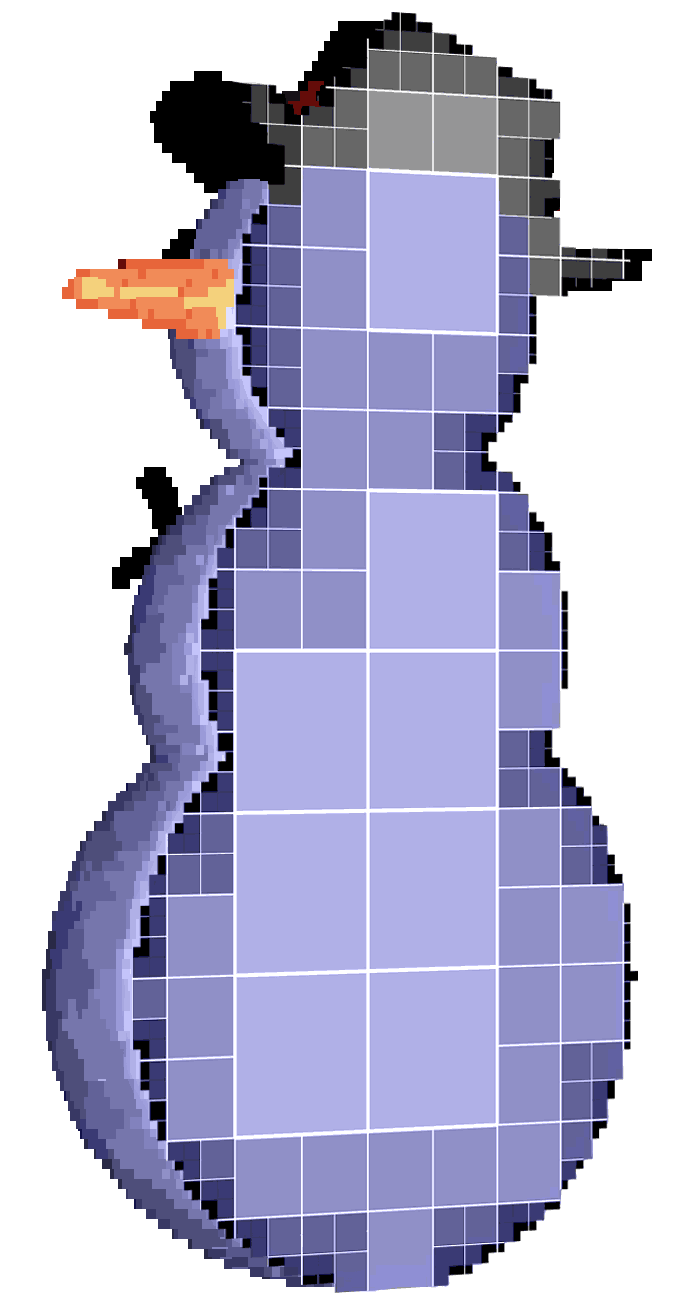
\includegraphics[scale=0.2]{obrazky-figures/svo_snowman.png}
	\caption{Ukázka reprezentace modelu pomocí sparse voxel octree}
	\label{fig:svo_example}
\end{figure}

\subsection{Light field probes}\label{sec:lfp_design}
Light field probes byly již krátce představeny v sekci \ref{sec:ray_tracing}. Každá sonda je reprezentována svou pozicí a texturou, která obsahuje následující informace:
\begin{itemize}
 \item Radiální vzdálenost ke geometrii.
 \item Normálu.
 \item Informace o materiálu, barvě či jiná data využitá v další práci se sondami.
\end{itemize}

Tato textura má velikost 1024x1024 a každý texel reprezentuje dvě float hodnoty (\texttt{rg32f}). Vzhledem k tomu, že paměťová náročnost je poměrně vysoká, je nutné ukládaná data nějakým způsobem komprimovat. Radiální vzdálenost ke geometrii je možné logaritmizovat pro zachování vyšší přesnosti pro bližší objekty a také kvantizovat na snížení paměťové náročnosti. Logaritmizace a linearizace hloubky je v rovnici \ref{eq:depth_econde_decode}.

\begin{equation} \label{eq:depth_econde_decode}
	\begin{gathered}
		encoded\_depth = \frac{log(C \cdot depth + 1)}{log(C \cdot Far)}\\
		decoded\_depth = \frac{(C \cdot Far + 1)^{encoded\_depth} - 1}{C}
	\end{gathered}
\end{equation}

Kde $C$ je konstanta modifikující rozložení přesnosti, často nastavena na 1, $depth$ je hloubka a $Far$ je maximální vzdálenost. Po logaritmizaci je hodnota transformována na 16 bitů a uložena do textury sondy.

Dalším parametrem jsou normály. Ty lze zakódovat na 2 float hodnoty mnoha metodami, jak je uvedeno v \cite{Cigolle2014ASO}. Zvolil jsem metodu projekce na osmistěn. Po projekci jsou složky výsledného vektoru kvantizovány na 8 bitů, čímž je celková potřebná paměť pro uložení těchto hodnot snížena na 16 bitů. Rovnice \ref{eq:normal_encode} popisuje zakódování normály a \ref{eq:normal_decode} její dekódování.

\begin{equation} \label{eq:normal_encode}
	\begin{gathered}
		\vec{p} = normal.xy \frac{1.0}{|normal.x| + |normal.y| + |normal.z|} \\
		\vec{encoded\_normal} = \begin{cases}
            (1.0 - |p.yx|) * sign(\vec{p}),& \text{pokud } normal.z \leq 0.0\\
            \vec{p},              & \text{jinak}
        \end{cases}\\
	\end{gathered}
\end{equation}

Kde $normal$ je normála, $p$ je pomocný vektor k projekci a $encoded\_normal$ je zakódovaná normála.

\begin{equation} \label{eq:normal_decode}
	\begin{gathered}
	    z = 1.0 - |encoded\_normal.x| - |encoded\_normal.y|\\
	    \vec{v} = \langle encoded\_normal.xy, z \rangle\\
		\vec{decoded\_normal} = \begin{cases}
            \langle (1.0 - |v.yx|) * sign(v.xy), v.z \rangle,& \text{pokud } v.z < 0.0\\
            normalize(\vec{v}),              & \text{jinak}
        \end{cases}\\
	\end{gathered}
\end{equation}

Kde $encoded\_normal$ je zakódovaná normála, $z$ je vypočtená třetí složka výsledné normály, $v$ je pomocný vektor a $decoded\_normal$ je dekódovaná normála.

Poslední položkou uloženou v textuře sondy je radiance. Pro případné další rozšíření je uložena ve formátu \texttt{R11G11B10} pro podporu HDR.

Jelikož sonda reprezentuje světelné pole ve svém okolí jakožto kouli, je nutné data nějakým způsobem transformovat na texturu, tedy rovinu. Toho lze dosáhnout mapováním koule na osmistěn a následné projekce na rovinu, jak je znázorněno na obrázku \ref{fig:octahedral_wrap}. Pro tuto projekci a její inverzní operaci je možné využít rovnic \ref{eq:normal_encode} a \ref{eq:normal_decode}.

\begin{figure}[H]
	\centering
	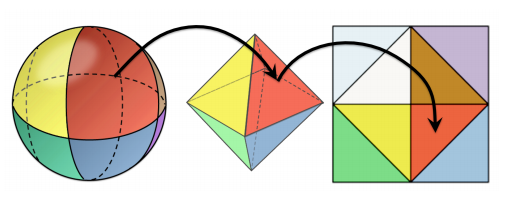
\includegraphics[scale=2]{images/octahedral_wrap.png}
	\caption{Vizualizace projekce na osmistěn a následně na rovinu}
	\label{fig:octahedral_wrap}
\end{figure}

Výpočet informací o geometrii je prováděn pomocí ray tracingu představeném v sekci \ref{sec:rendering}. Na obrázku \ref{fig:probe_in_scene} je ukázka dat jedné ze sond.


\begin{figure}[H]
	\centering
	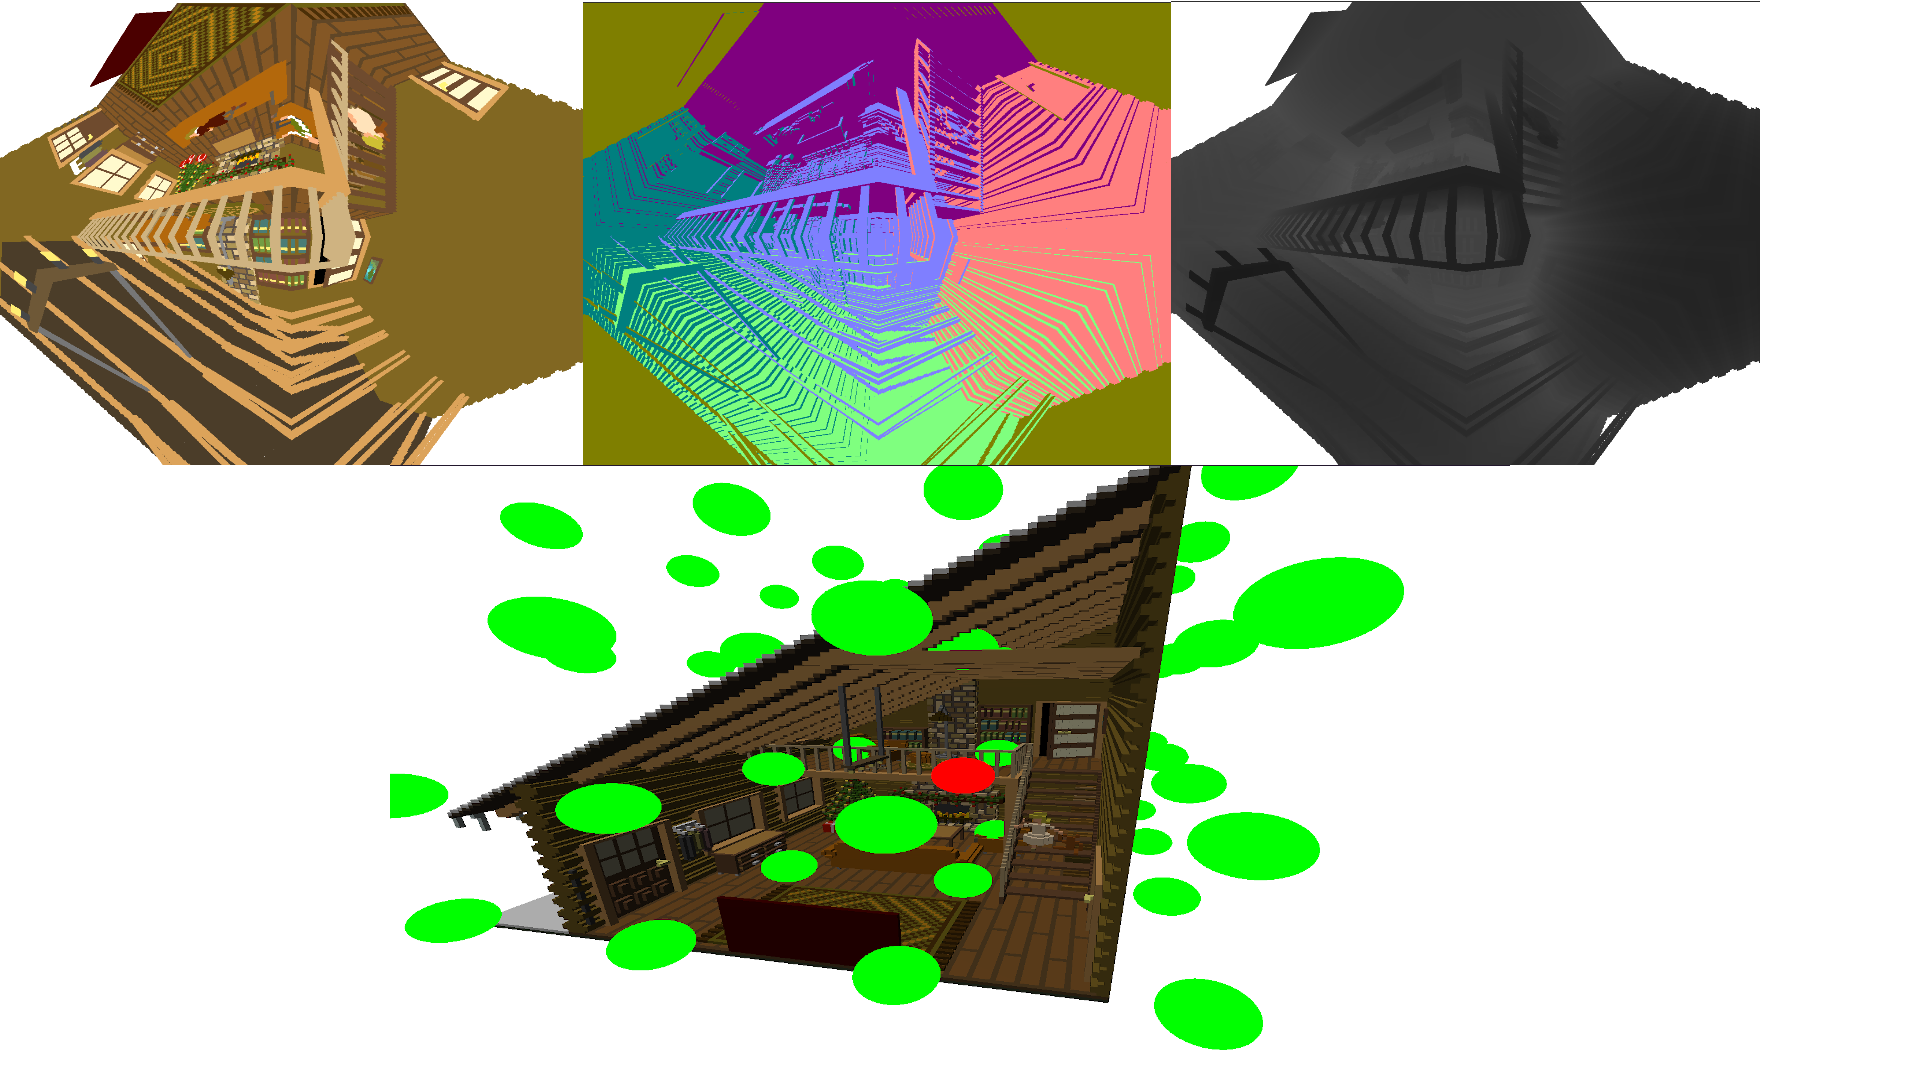
\includegraphics[scale=1]{images/probe_with_scene.png}
	\caption{Vizualizace dat uložených pro sondu (horní část v pořadí radiance, normály, hloubka) a její pozice ve scéně (dolní část, červená koule je zobrazovaná sonda)}
	\label{fig:probe_in_scene}
\end{figure}

\subsection{Renderování scény pomocí light field probes}
Pomocí atlasu textur, který byl vytvořen pro všechny sondy pokrývající scénu, je možné provádět trasování paprsku. Tato metoda byla popsána v publikaci \cite{light_field_probes}. Díky radiální vzdálenosti a normálám zakódovaných v sondách můžeme vypočítat průsečíky nesouvislých paprsků. 

V prvé řadě je nutné pro paprsek vybrat vhodnou sondu, ve které zahájíme jeho sledování. Pokud tato sonda není schopná poskytnout nám jistý \textit{miss} (minutí scény) nebo \textit{hit} (protnutí scény) je nutné vybrat alternativní sondu, která má nějakou šanci paprsek sledovat. Sledování paprsku v rámci jedné sondy tedy vrací tři stavy:
\begin{itemize}
    \item \textit{miss} -- minutí scény
    \item \textit{hit} -- průsečík se scénou
    \item \textit{unknown} -- neznámý výsledek
\end{itemize}

Stav \textit{unknown} nastane pouze v případě, kdy paprsek prochází ve větší vzdálenosti, než jaká je v daná pozici radiální hloubka. Jinými slovy, pokud sonda "ví", že nemá dostatečné informace o scéně v dané pozici, nemůže být paprsek spolehlivě vyhodnocen pouze pomocí informací z této sondy. 

Sledování paprsku začíná jeho převedením jeho počátku do prostoru sondy, následně je paprsek transformován pomocí projekce na osmistěn do souřadnic textury. Dochází tedy k transformaci přímky z $R^3$ do křivky v $R^2$. Tato křivka má až čtyři segmenty, kde každý segment leží v jiné stěně osmistěnu. Následně algoritmus postupuje po jednotlivých texelech nacházejících se na této křivce a vyhodnocuje, jestli dochází k průsečíku pomocí porovnávání uložené hloubkové mapy se vzdáleností paprsku k sondě. Pokud je paprsek ve stejné vzdálenosti, nebo je dále, dochází k průsečíku nebo paprsek prochází za geometrií. Algoritmus pro výpočet průsečíku je v algoritmu \ref{alg:single_probe_trace}. 

\begin{center}
	\begin{czechalgorithm}[H] \label{alg:single_probe_trace}
	    segments = compute\_segments(ray, probe)\\
	    \ForEach{segment in segments}{
	        coords\_on\_segment = create\_coords(segment)\\
	        \ForEach{coord in coords\_on\_segment}{
	            state = compare\_ray\_distance\_to\_radial(ray, coord, probe)\\
	            \uIf{state == HIT}{
	                \KwRet (HIT, coord)
	            }
	            \uIf{state == HIDDEN\_BEHIND\_SURFACE}{
	                \KwRet (UNKNOWN, coord) 
	            }
	        }
	    }
	    \KwRet (MISS, last\_point\_on\_segments)
		\caption{Sledování paprsku v rámci jedné sondy}
	\end{czechalgorithm}
\end{center}

Pro urychlení tohoto algoritmu je pro každou sondu vytvořena další textura, která má 16-krát menší velikost -- tedy 64x64 -- ve které jsou uloženy v každém texelu nejbližší radiální vzdálenosti. Jedná se prakticky o mipmapu. Při procházení pixelů segmentů tedy není nutné provádět algoritmus na maximálním rozlišení, čímž dochází k výraznému zrychlení. Pouze při nalezení potenciálního průsečíku je trasování prováděno na vysokém rozlišení. Na obrázku \ref{fig:lfp_trace} je vizualizace průchodu paprsku jednou sondou.

\begin{figure}[H]
	\centering
	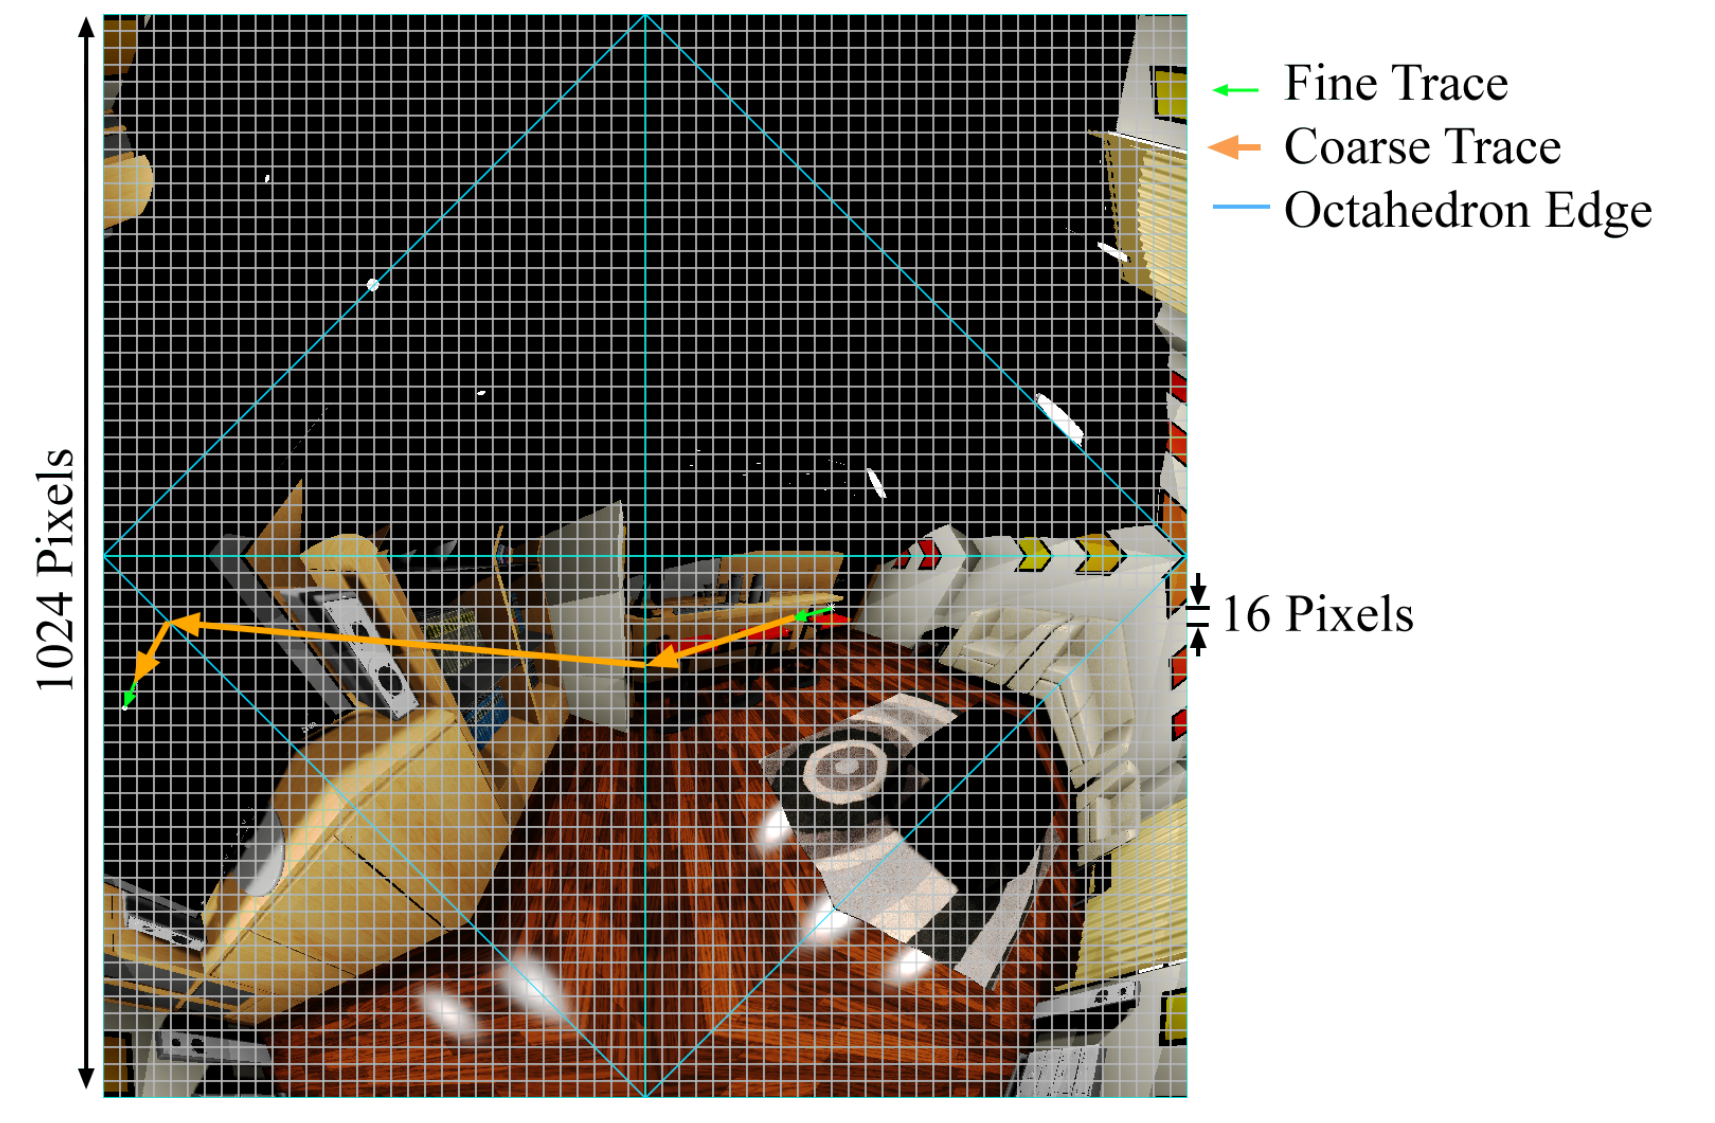
\includegraphics[scale=1]{images/lfp_trace.png}
	\caption{Vizualizace sledování paprsku v textuře sondy. Oranžová část je prováděna pouze na textuře s nižším rozlišením, zelená při nalezení potenciálního průsečíku}
	\label{fig:lfp_trace}
\end{figure}

\paragraph{Výběr sondy.} Samozřejmě nejdůležitějším krokem je výběr vhodné sondy pro zahájení algoritmu. Jedním možným řešením je výběr sondy čistě podle vzdálenosti k počátku paprsku, což doporučuje taktéž článek \cite{light_field_probes}, s tím, že výběr dalších sond se řídí pořadím uvedeným v obrázku \ref{fig:lfp_cube}. Pokud se paprsek nenachází v jiné skupině sond po dokončení průchodu této skupiny je hledání ukončeno jako neúspěšné, jinak je prováděno v nové skupině. V mém případě docházelo k velkému množství \textit{unknown} výsledků a proto jsem se rozhodl implementovat jiné řešení. 

\begin{figure}[H]
	\centering
	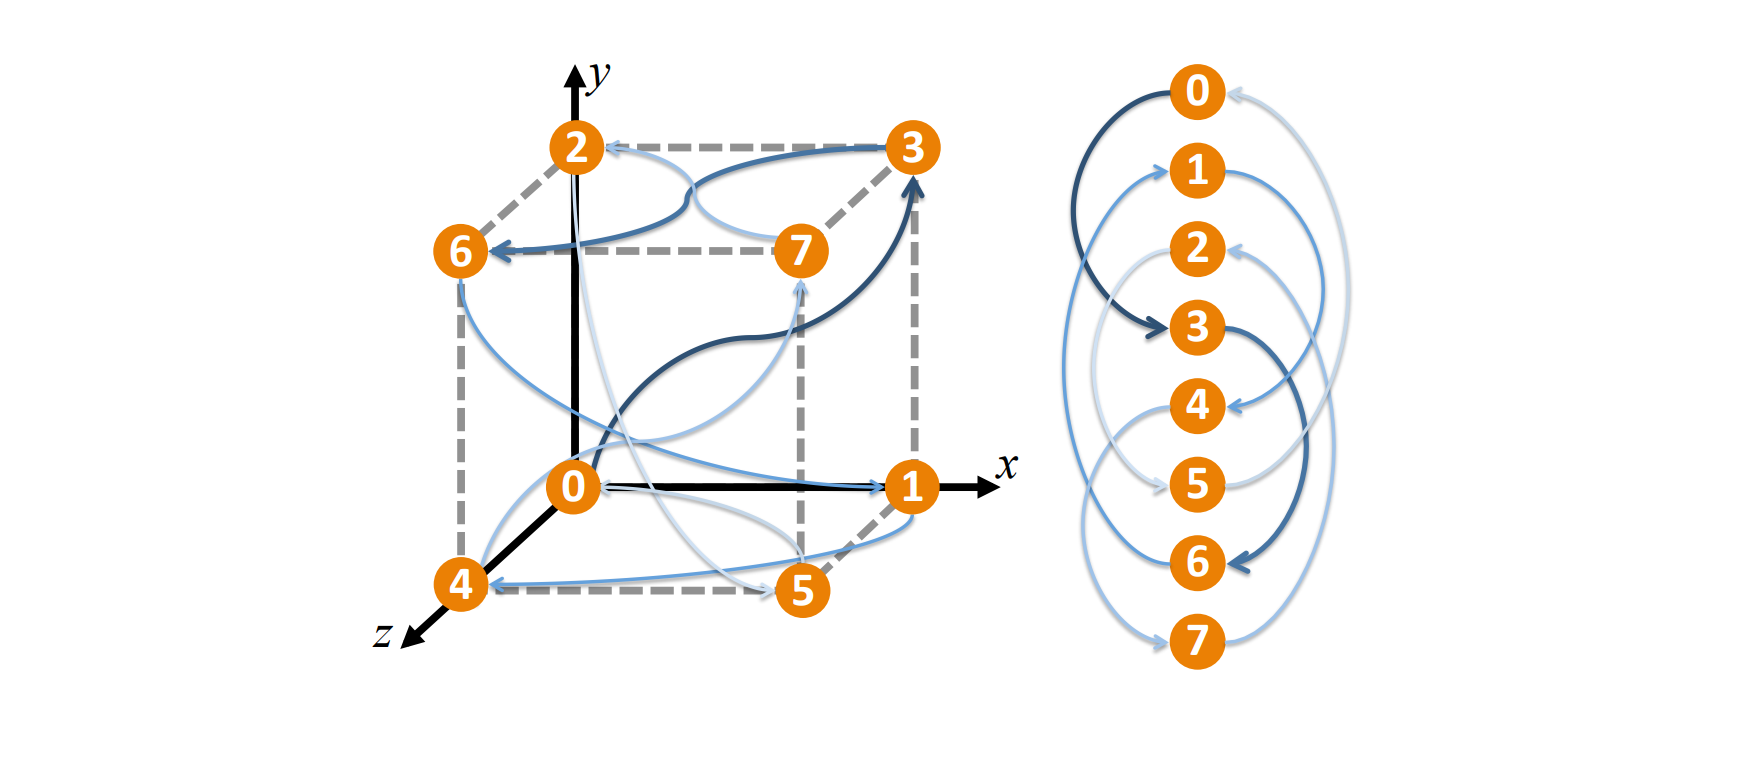
\includegraphics[scale=1]{images/probe_cube.png}
	\caption{Pořadí výběru sondy pro lokální skupinu}
	\label{fig:lfp_cube}
\end{figure}

Namísto výběru sondy tak, jak je popsáno v předchozím odstavci, je možné rozdělit prostor, který je sondami sledován, na voxelové pole (mřížku). Toto pole obsahuje pro každý voxel až čtyři sondy, pro které se daný voxel vyskytuje blíže, než je jejich radiální vzdálenost ke scéně. Namísto výběru nejbližší sondy tedy vybereme sondu podle toho, ve kterém voxelu se paprsek současně nachází. Sledování ukončíme pouze tehdy, pokud žádná ze sond uložená v tomto poli nenalezla řešení a sledovaný bod paprsku se neposunul do jiného voxelu. 

\begin{center}
	\begin{czechalgorithm}[H] \label{alg:light_field_trace}
	    result = UNKNOWN\\
	    \While{result == UNKNOWN}{
	        probe = select\_probe\_from\_voxel\_field(ray)\\
	        \uIf{\Not is\_valid\_probe(probe)}{
	            break
	        }
	        (result, endpoint) = trace\_single\_probe(ray, probe)\\
	        ray.origin = endpoint
	    }
	    \KwRet result
		\caption{Sledování paprsku skrze light field}
	\end{czechalgorithm}
\end{center}

Na obrázku \ref{fig:lfp_scene_render} je zobrazena scéna vykreslená čistě pomocí výše popsané metody. Zelené oblasti značí \textit{miss}, červené \textit{unknown}. Je vidět, že dochází k mnoha nepřesnostem a ve scéně, kde je spousta objektů dochází ke vzniku míst, kde sondy nenaleznou řešení.

\begin{figure}[H]
	\centering
	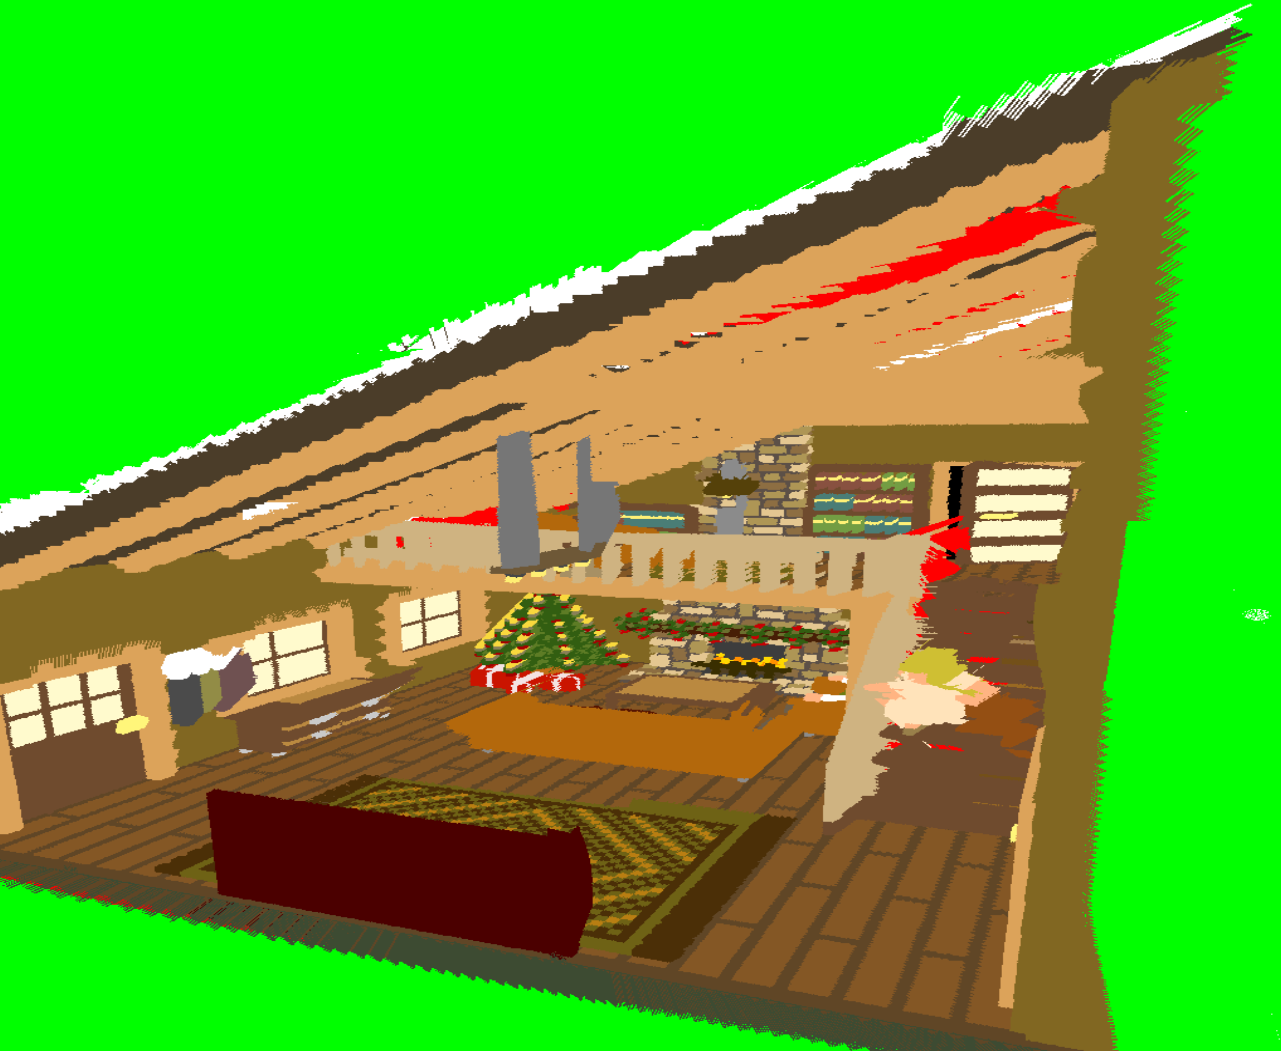
\includegraphics[scale=1]{images/probe_scene_render.png}
	\caption{Scéna vykreslena pomocí sledování paprsku skrze light field}
	\label{fig:lfp_scene_render}
\end{figure}

\subsection{Nepřímé osvětlení}
Mým původním záměrem bylo využít výše popsané sondy k výpočtu sekundárních paprsků ve scéně online, ale ukázalo se, že pro takový přístup je tato metoda příliš pomalá. Bylo tedy nutné vymyslet alternativní řešení. 

Pro již zmíněnou metodu se nabízí modifikace, která by umožnila přidat funkčnost nepřímého osvětlení tak, že do atlasu textur sond vypočteme nepřímé osvětlení při jejich inicializaci a posléze je aplikujeme při renderování scény.  K výpočtu použijeme ray tracing implementovaný pomocí metody popsané v první části sekce. Pro každý texel, který reprezentuje difuzní materiál, je vysláno několik paprsků z místa prvního průsečíku scény. Tyto paprsky se dále odráží ve scéně a sbírají světlo z vnějších zdrojů/emitujících materiálů.


\begin{figure}[H]
	\centering
	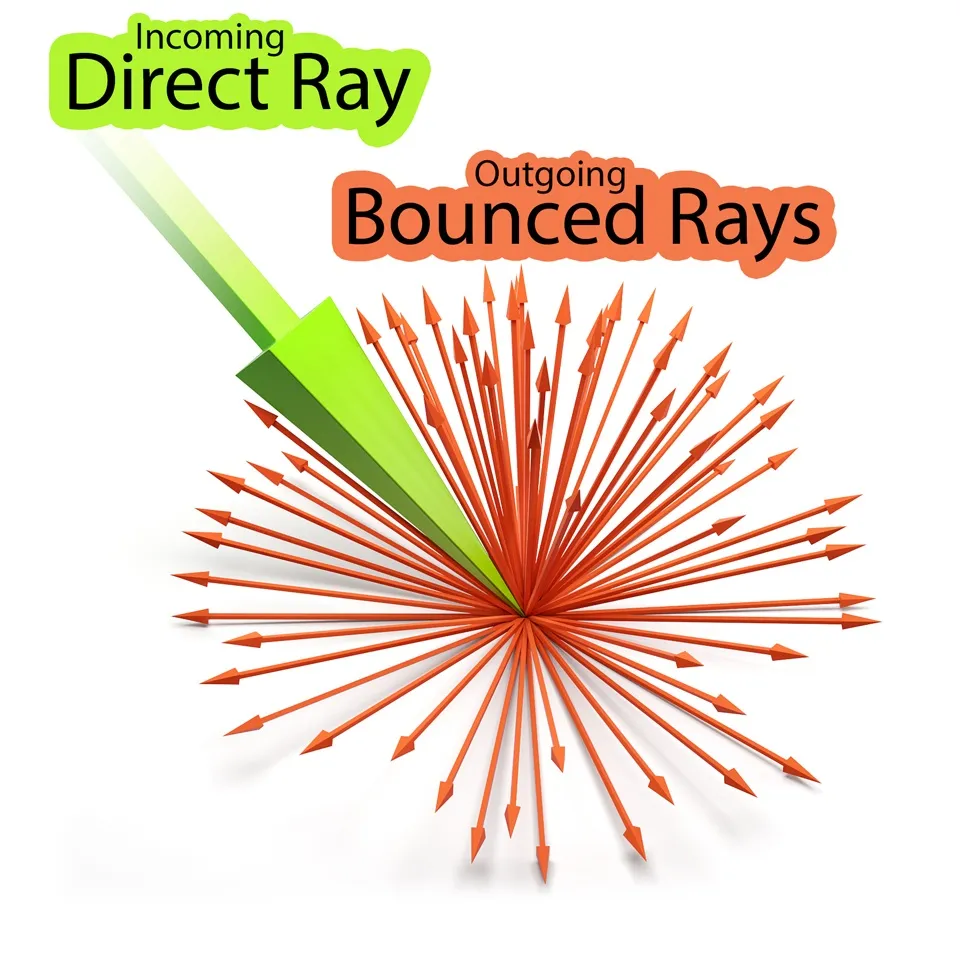
\includegraphics[scale=0.15]{images/diffuse_bounce.png}
	\caption{Paprsky odražené z difuzního materiálu}
	\textbf{Zdroj: \url{https://renderstuff.com/tutorials/indirect-illumination-in-v-ray-tutorial-176/}}
	\label{fig:diffuse_rays}
\end{figure}


Jelikož informace o materiálech poskytované zdrojovými modely jsou poměrně stručné, odraz paprsku je prováděn náhodně v polokouli určené normálou, jak je demonstrováno na obrázku \ref{fig:diffuse_rays}. Výpočet příspěvku osvětlení je popsán v algoritmu \ref{alg:bounce_bake}.

\begin{center}
	\begin{czechalgorithm}[H] \label{alg:bounce_bake}
	    result = vector(1, 1, 1)\\
	    \For{i in range(0, MAX\_BOUNCES)}{
	        (is\_hit, position, normal, material\_type) = trace\_ray(ray)\\
	        \uIf{\Not is\_hit}{
	            break
	        }
	        \uIf{material\_type == DIFFUSE}{
	            result *= attentuation\\
	            ray.origin = position\\
	            ray.direction = random\_point\_on\_hemisphere(normal)
	        }
	        \uIf{material\_type == METALLIC}{
	            ray = bounce\_ray\_for\_metallic(ray, position, normal)\\
	        }
	        \uIf{material\_type == EMIT}{
	            add\_emissive\_light(result)\\
	            break
	        }
	    }
	    \KwRet result
		\caption{Výpočet nepřímého osvětlení}
	\end{czechalgorithm}
\end{center}

\begin{figure}[H]
	\centering
	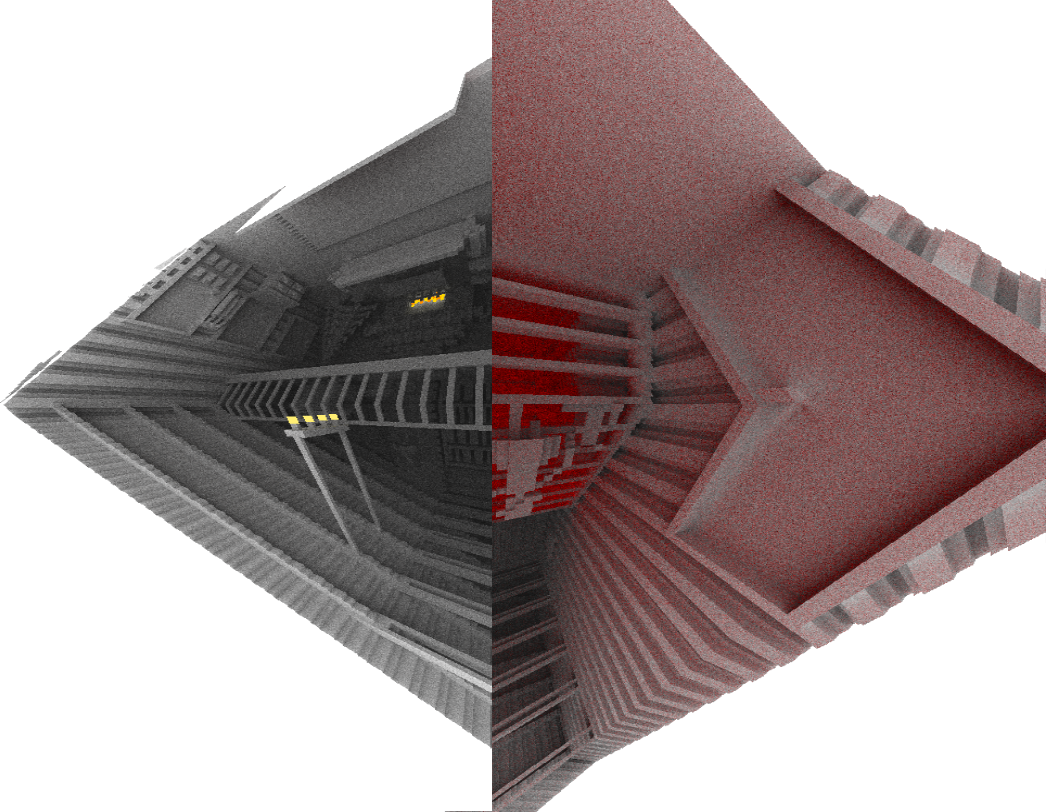
\includegraphics[scale=1]{images/indirect_probe.png}
	\caption{Textura sondy obsahující informace o nepřímém osvětlení. Na levé straně pouze vnější osvětlení, vpravo vliv emitujícího materiálu.}
	\label{fig:diffuse_rays}
\end{figure}


\section{Struktura vykreslovacího řetězce}


\chapter{Implementace}
\label{implementace}

Tato kapitola obsahuje seznam použitých nástrojů a knihoven. Popisuje implementaci knihoven vytvořených při práci na praktické části tohoto projektu, také algoritmy použité ke tvorbě octree a uživatelské rozhraní demonstrační aplikace.

\section{Použité knihovny a nástroje}
Pro implementaci jsem zvolil jazyk \texttt{c++}, standard 20\footnote{\url{https://en.cppreference.com/w/cpp/20}}, kvůli mé pokročilé znalosti jazyka a také jako možnost procvičit si nově přidané funkce v~poslední revizi. Pro překlad projektu jsem použil \texttt{CMake}\footnote{\url{https://cmake.org/}} v~kombinaci s~\texttt{Ninja}\footnote{\url{https://ninja-build.org/}} a package management nástroji \texttt{CPM.cmake}\footnote{\url{https://github.com/TheLartians/CPM.cmake}} a \texttt{Hunter}\footnote{\url{https://hunter.readthedocs.io/en/latest/}}. Jako vývojové prostředí jsem využil \texttt{CLion}\footnote{\url{https://www.jetbrains.com/clion/}}. Kód shaderů je vytvořen v~GLSL\footnote{\url{https://www.khronos.org/opengl/wiki/Core_Language_(GLSL)}}. Při práci na projektu jsem také využil tyto knihovny třetích stran:

\begin{itemize}
	\begin{AutoMultiColItemize}
		\item \texttt{spdlog}\footnote{\url{https://github.com/gabime/spdlog}}
		\item \texttt{range-v3}\footnote{\url{https://github.com/ericniebler/range-v3}}
		\item \texttt{magic\_enum}\footnote{\url{https://github.com/Neargye/magic_enum}}
		\item \texttt{argparse}\footnote{\url{https://github.com/p-ranav/argparse}}
		\item \texttt{toml++}\footnote{\url{https://marzer.github.io/tomlplusplus/}}
		\item \texttt{backward-cpp}\footnote{\url{https://github.com/bombela/backward-cpp}}
		\item \texttt{cppcoro}\footnote{\url{https://github.com/lewissbaker/cppcoro}}
		\item \texttt{\{fmt\}}\footnote{\url{https://github.com/fmtlib/fmt}}
		\item \texttt{stb}\footnote{\url{https://github.com/nothings/stb}}
		\item \texttt{glm}\footnote{\url{https://github.com/g-truc/glm}}
		\item \texttt{Dear ImGui}\footnote{\url{https://github.com/ocornut/imgui}}
	\end{AutoMultiColItemize}
\end{itemize}

Dále jsem použil následující nástroje pro statickou analýzu kódu, formátování atp.:
\begin{itemize}
	\begin{AutoMultiColItemize}
		\item \texttt{cppcheck}\footnote{\url{http://cppcheck.sourceforge.net/}}
		\item \texttt{cpplint}\footnote{\url{https://github.com/cpplint/cpplint}}
		\item \texttt{sanitisers}\footnote{\url{https://github.com/google/sanitizers}}
		\item \texttt{valgrind}\footnote{\url{https://valgrind.org/}}
		\item \texttt{Ccache}\footnote{\url{https://ccache.dev/}}
		\item \texttt{clang-format}\footnote{\url{https://clang.llvm.org/docs/ClangFormat.html}}
	\end{AutoMultiColItemize}
\end{itemize}

\section{Knihovna pf\_common}
Knihovna poskytující často používané funkce:
\begin{itemize}
	\item \texttt{Concept}y a další nástroje pro template meta programování a statický polymorfimus.
	\item Jednoduché coroutines (\texttt{iota}, \texttt{range}...)
	\item Implementace výjimek se stack trace reporting.
	\item Některé idiomy \texttt{c++} -- \texttt{RAII}, \texttt{Visitor}...
	\item Funkce pro binární serializaci dat a práci s~binárními daty.
	\item Obecné geometrické funkce, které nejsou poskytnuty v \texttt{glm}.
	\item Funkce pro rozšíření možnosti využití \texttt{enum}.
	\item Mnoho dalších...
\end{itemize}

Je implementována jako header-only knihovna\footnote{\url{https://en.wikipedia.org/wiki/Header-only}}.

\section{Knihovna pf\_glfw\_vulkan}
Tato knihovna poskytuje dvě základní funkce:
\begin{itemize}
	\item vytvoření a správa okna pomocí \texttt{GLFW}\footnote{\url{https://www.glfw.org/}}
	\item komunikace s~GPU za pomocí \texttt{Vulkan API}\footnote{\url{https://www.khronos.org/vulkan/}}
\end{itemize}

Třída \texttt{GlfwWindow} umožňuje instanciaci GLFW knihovny a také komunikaci za pomocí událostí, které knihovna programu předává. Umožňuje uživateli interagovat s aplikací za pomocí periferních zařízení (myš a klávesnice). Tato třída splňuje concept\footnote{\url{https://en.cppreference.com/w/cpp/language/constraints}} \texttt{Window}, který je také obsažen v~knihovně. Za pomocí \texttt{Window} je implementována komunikace mezi \texttt{Vulkan} a okenním systémem - díky tomuto rozdělení si může uživatel vytvořit komunikační vrstvu mezi knihovnou a jiným okenním systémem, jako například \texttt{SDL}\footnote{\url{https://www.libsdl.org/}}. Pro tento účel implementuje knihovna vlastní notifikační systém událostí ve třídě \texttt{EventDispatchImpl}, který výrazně usnadňuje případnou implementaci s jiným okenním backendem.

Část knihovny pro interakci s~\texttt{Vulkan} je o~poznání rozsáhlejší. Při návrhu knihovny byl kladen zřetel především na její jednoduchost a zároveň bezpečnost jejího užívání. Z~tohoto důvodu je uvnitř hojně využito \texttt{std::shared\_ptr}. Vzhledem k~tomu, že ve \texttt{Vulkan} často musíme vytvářet objekty v~závislosti na některém z dříve vytvořených (například \texttt{vk::Instance} $\longrightarrow$ \texttt{vk::PhysicalDevice} $\longrightarrow$ \texttt{vk::Device}) si v~sobě každý nově vytvořený potomek ukládá ukazatel na svého "rodiče". To zaručuje, že nemůže dojít k~uvolnění objektů omylem, v případě, že budeme používat některého z~jeho potomků.

Knihovna obsahuje vlastní verzi velkého množství \texttt{Vulkan} objektů a zároveň je plně typově bezpečná. Příkladem může být přístup do \texttt{vk::Buffer}, kdy k~datům přistupujeme pomocí mapovacího objektu, který hojně využívá template funkcí pro kontrolu offsetu a správné práce s~pamětí.

Všechny objekty jsou potomkem \texttt{VulkanObject}, což je rozhraní, které poskytuje základní debug informace o~objektu. Vytváření objektů je vždy prováděno pomocí \texttt{struct} konfiguračních dat. Předpokládá se užití \texttt{designated initialisers}\footnote{\url{https://en.cppreference.com/w/cpp/language/aggregate_initialization#Designated_initializers}}. Ukázka vytvoření logického zařízení:

\begin{lstlisting}[language=C++, caption={Tvorba logického zařízení}]
// tvorba instance vynechana kvuli velkemu mnozstvi argumentu
device = instance->selectDevice(DefaultDeviceSuitabilityScorer());
surface = instance->createSurface(window);
logicalDevice = device->createLogicalDevice({
    .id = "dev1",
    .deviceFeatures = vk::PhysicalDeviceFeatures{},
    .queueTypes = {vk::QueueFlagBits::eCompute},
    .presentQueueEnabled = true,
    .requiredDeviceExtensions = {VK_KHR_SWAPCHAIN_EXTENSION_NAME},
    .validationLayers = getValidationLayers(),
    .surface = *surface});
\end{lstlisting}

Pro objekty, u~nichž by konfigurační struktura vyžadovala nadměrně velké množství argumentů, jsou v~knihovně dostupné builder třídy, například \texttt{GraphicsPipelineBuilder} nebo \texttt{RenderPassBuilder}.

Součástí knihovny je též rozhraní pro kompilaci shader souborů z disku nebo paměti.



\section{Knihovna pf\_imgui}\label{sec:pf_imgui}
\texttt{pf\_imgui} je event-driven UI knihovna postavena na Dear Imgui. Cílem je zjednodušení práce při vytváření uživatelského rozhraní a také přidání některých funkcí. Funkce, které jsou oproti Dear Imgui přidané jsou:

\begin{itemize}
	\item Pozorování změn hodnot pomocí callback funkcí (observer pattern).
	\item Ukládání hodnot do konfiguračního souboru. Tyto změny jsou načteny vždy při zapnutí programu.
	\item Některé elementy navíc, například \texttt{Memo}.
\end{itemize}

Knihovna je postavena nezávisle na renderovacím backendu, v repository je poskytnut backend pro \texttt{Vulkan} a \texttt{GLFW}. Pro vlastní použití je nutné rozšířit hlavní objekt \texttt{ImGuiInterface} a přidat volání do backendu své volby. Například pro \texttt{Vulkan} by se mohlo jednat o~jednoduchou funkci přidání draw command do \texttt{vk::CommandBuffer}. V~knihovně je obsaženo podstatné množství elementů, přičemž jsou implementovány wrappery pro všechny elementy dostupné v~Dear Imgui. Také jsou přidány grafy z~knihoven \texttt{ImGuiFlameGraph}\footnote{\url{https://github.com/bwrsandman/imgui-flame-graph}}, \texttt{implot}\footnote{\url{https://github.com/epezent/implot}} a možnost interagovat se soubory na disku pomocí \texttt{ImGuiFileDialog}\footnote{\url{https://github.com/aiekick/ImGuiFileDialog}}.

V knihovně je také implementováno podstatné množství layoutů -- grid layout, anchor layout...

Přidání vlastních elementů do knihovny je velice primitivní. Připravená rozhraní pokrývají spoustu potenciální funkčnosti včetně například \texttt{drag and drop} a rozhraní pro nastavení stylu/ barvy elementu. 

Například implementace \texttt{CheckBox} vyžaduje jen \textasciitilde10 řádků kódu -- nepočítaje deklarace funkcí a tělo konstruktoru -- s~tím, že dědí z~\texttt{ItemElement}, \texttt{Labellable}, \texttt{Savable}, \texttt{ValueObservable<bool>}, \texttt{ColorCustomizable<...>} a \texttt{StyleCustomizable<...>}.

Ukázka vytvoření tlačítka, které reaguje na kliknutí otevřením dialogu pro výběr \texttt{txt} souboru:

\begin{lstlisting}[language=C++, caption={Vytvoření tlačítka pro výběr souboru}]
imgui.createChild<Button>("btn_id", "Open file")
    .addClickListener([&imgui] {
        imgui.openFileDialog("Select file", 
            {.ext = {"txt"}, .description = "txt  files"}, 
            [] (const auto &files) {
                for (const auto &file : files) { print(file); }
            }, [] { print("No file selected"); });
    }
\end{lstlisting}


\section{Načítání modelů a jejich transformace} \label{sec:voxel_conversion}
Pro vykreslování modelů je nutné je transformovat do octree. Jelikož neexistuje žádný standardní formát pro voxely, je potřeba implementovat import pro různé formáty. Aplikace je prozatím schopna importovat formát \texttt{vox} (sekce \ref{sec:format})).

Načítání dat je rozděleno na dvě části. V~první části jsou ze vstupního souboru načteny využité materiály a je vytvořen seznam voxelů. Tohle je jediná část, kterou je nutné implementovat speciálně pro nové formáty. Zbytek převodu je popsán v~algoritmu \ref{alg:vox_to_svo}.


\begin{center}
	\begin{czechalgorithm}[H] \label{alg:vox_to_svo}
		voxels.sort() \\
		tree\_depth = calculate\_tree\_depth(voxels)\\
		root = tree.init\_root()\\
		\ForEach{voxel in voxels}{
			node = root\\
			\For{level = 0; level < tree\_depth; level++} {
				index\_for\_level = getIndexForLevel(voxel.position, level, tree\_depth)\\
				child\_node = node.get\_or\_create\_node(index\_for\_level)\\
				// nastaveni hodnot voxelu (material...)\\
				node = child\_node\\
			}
			node.is\_terminal = true\\
		}
		\caption{Převod voxelů do octree}
	\end{czechalgorithm}
\end{center}

Po vytvoření stromové reprezentace je dalším krokem minimalizace stromu. Pokud jsou některé oblasti zaplněné, můžeme snížit jeho složitost - označíme uzel na vyšší úrovni jako terminální a jeho potomky odstraníme.

\begin{center}
	\begin{czechalgorithm}[H] \label{alg:minimize_svo}
		\SetKwFunction{FMinTree}{MinimizeTree}
		\SetKwFunction{FIsFilled}{IsNodeFilled}
		\SetKwProg{Fn}{Function}{:}{}

		\Fn{\FIsFilled{$node$}}{
			\KwRet $node$.child\_count == 8 \&\& all\_of($node$.children, IsFilled)\\
		}

		\Fn{\FMinTree{$node$}}{
			\uIf{IsNodeFilled($node$)}{
				node.children.clear()\\
				node.is\_terminal = true\\
			}
			\uElse{
				\ForEach{child in $node$.children}{
					MinimizeTree(child)\\
				}
			}
		}
		\caption{Minimalizace octree}
	\end{czechalgorithm}
\end{center}

\begin{figure}[H]
	\centering
	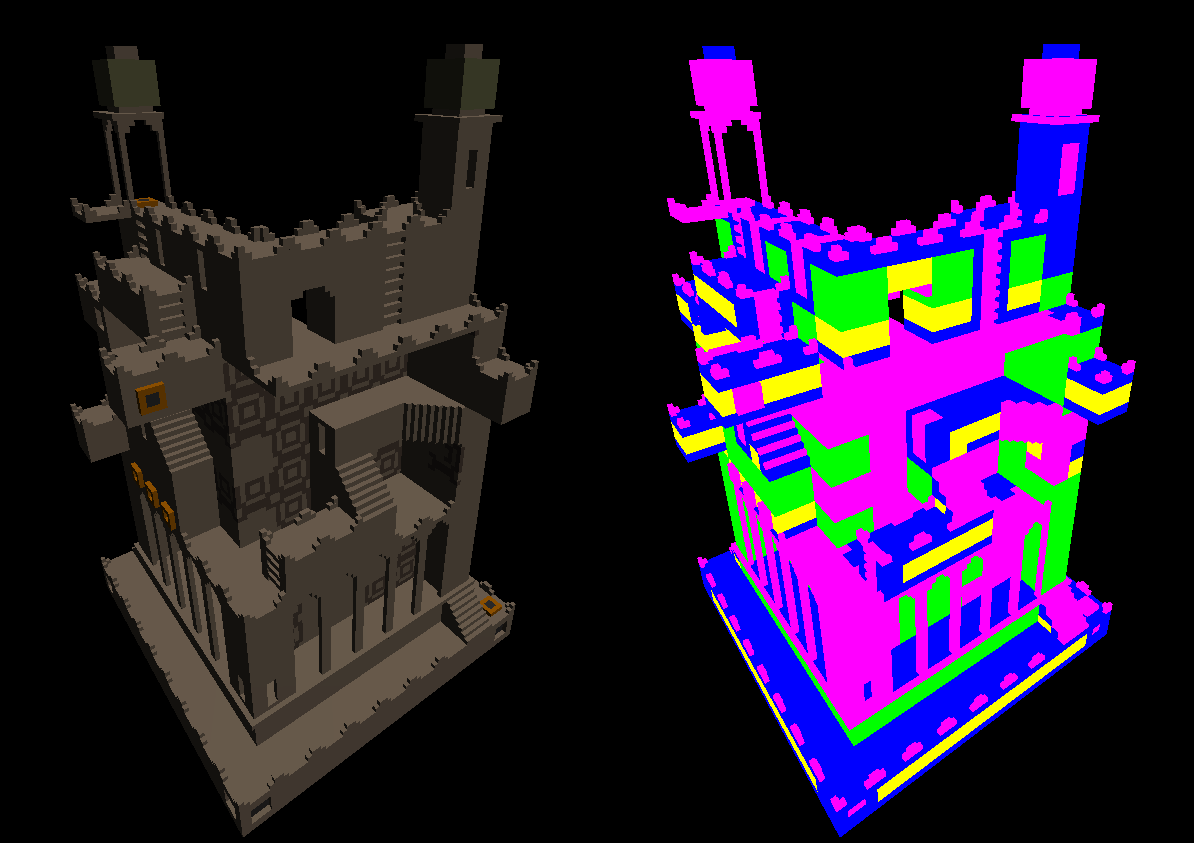
\includegraphics[scale=0.7]{obrazky-figures/levels_render.png}
	\caption{Vizualizace voxelů podle jejich hloubky ve stromu, vlevo render, vpravo barevně odlišené úrovně}
	\label{fig:imgui_classes}
\end{figure}



Finálním krokem je transformace vytvořeného stromu do jeho binární reprezentace popsané v~sekci \ref{sec:voxel_representation}.


\section{Výpočet průsečíku se scénou} \label{sec:bvh_traversal_impl}
Paprsky vycházející z kamery jsou generováno 

Algoritmus \ref{alg:traverse_bvh_impl} popisuje průchod BVH stromem za využití zásobníku. Důležitou součástí tohoto algoritmu je řazení potomků uzlu podle jejich vzdálenosti od počátku paprsku. Díky tomu jsou uzly stromu procházeny v pořadí od nejbližšího, můžeme tedy od určité chvíle naprosto ignorovat modely, jejichž obalové těleso (AABB) se nachází dále než prozatím nejbližší průsečík scény. Je zde také menší pravděpodobnost, že bude docházet k větvení kvůli pořadí průchodu.

\begin{center}
	\begin{czechalgorithm}[H] \label{alg:traverse_bvh_impl}
	    \SetKw{Or}{\hspace{\algoskipindent}\itshape or\;}
        \SetKw{And}{\hspace{\algoskipindent}\itshape and\;}
        \SetKw{Not}{\itshape not}
		\SetKwFunction{FTraverseBVH}{TraverseBVH}
		\SetKwFunction{FIntersectNode}{IntersectNode}
		\SetKwProg{Fn}{Function}{:}{}

		\Fn{\FTraverseBVH{$ray$}}{
		    best\_model\_intersection\_distance = INFINITY\\
		    intersection\_a = IntersectNode(root)\\
		    stack = EmptyStack()\\
		    \While{intersection\_a.hit}{
		       \While{\Not intersection\_a.is\_leaf \And intersection\_a.hit}{
		            intersection\_a = IntersectNode(intersection\_a.node.left\_child)\\
		            intersection\_b = IntersectNode(intersection\_a.node.right\_child)\\
		            \uIf{intersection\_a.distance < instersection\_b.distance}{
		                swap(intersection\_a, intersection\_b)
		            }
		            \uIf{intersection\_b.hit \And intersection\_b.distance < best\_model\_intersection\_distance}{
		                stack.Push(intersection\_b)
		            }
		            \uIf{\Not intersection\_a.hit \And \Not stack.Empty()}{
		                intersection\_a = stack.Pop()
		            }
		        }
			}
		    
    		\uIf{intersection\_a.is\_leaf}{
    		    \uIf{intersection\_a.distance < best\_model\_intersection\_distance}{
    		        model\_intersection = TraceModel(intersection\_a.model\_id\\
    		        \uIf{model\_intersection.hit \And model\_intersection.distance < best\_model\_intersection\_distance}{
    		            best\_model\_intersection\_distance = model\_intersection.distance 
    		        }
    		    }
    		}
    		\eIf{stack.Empty()}{
    		    intersection\_a.hit = false
    		} {
    		    intersection\_a = stack.Pop()
    		}
		}
		\caption{Průchod paprsku hierarchií obalových těles}
	\end{czechalgorithm}
\end{center}

\section{Demonstrační aplikace}
Demonstrační aplikace slouží k vizualizaci výsledků a práci s modely/scénami. Aplikace může pracovat ve dvou režimech:
\begin{itemize}
    \item Editační režim -- v tomto režimu je scéna vykreslována pouze pomocí sparse voxel octree ray marchingu a slouží primárně k vytvoření scény a jejímu uložení na disk. Také je lze možné sledovat stav sond.
    \item Renderovací režim -- slouží k načítání scén vytvořených v předchozím režimu a demonstraci výsledného algoritmu.
\end{itemize}

Uživatelské rozhraní je implementováno pomocí knihovny \texttt{pf\_imgui} představené v sekci \ref{sec:pf_imgui}. Většina prvků uživatelského rozhraní obsahuje tooltipy pro snadné zjištění funkce jednotlivých komponent a UI okna lze přetáhnout ven z hlavního okna pro lepší přehlednost. Bližší popis se nachází na přiloženém paměťovém médiu, základní přehled zde ale bude uveden.

\begin{figure}[H]
	\centering
	\captionsetup{justification=centering}
	\begin{subfigure}[t]{.49\textwidth}
		\centering
		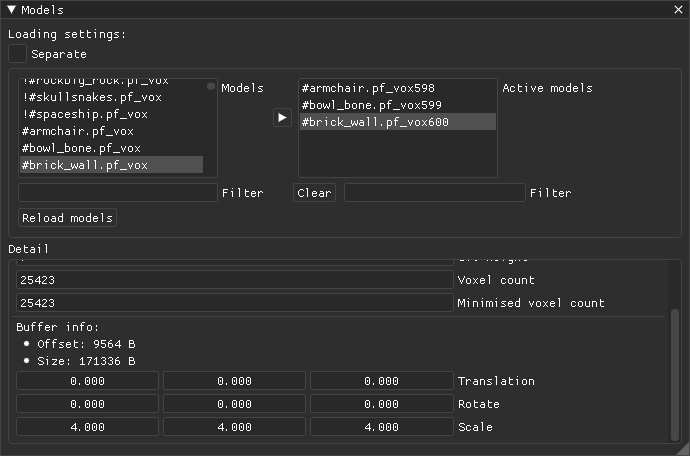
\includegraphics[scale=1]{images/dp_ui_models.png}
		\caption{\textbf{Okno pro přidávání a manipulaci s modely}}
		\label{fig:model_ui}
	\end{subfigure}
		\begin{subfigure}[t]{.49\textwidth}
		\centering
		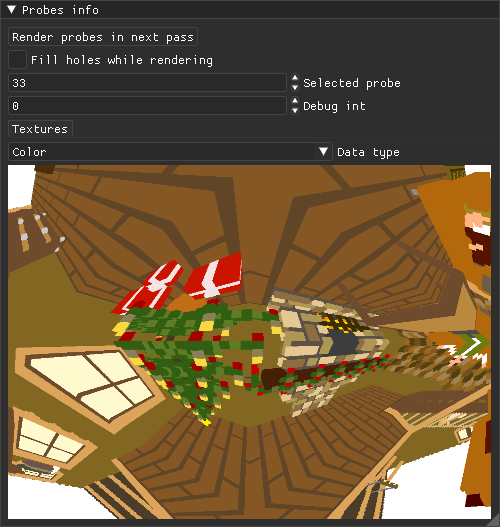
\includegraphics[scale=1]{images/dp_ui_probes.png}
		\caption{\textbf{Okno pro zobrazení atlasu textur sond}}
		\label{fig:probe_ui}
	\end{subfigure}
		\begin{subfigure}[t]{1\textwidth}
			\centering
        	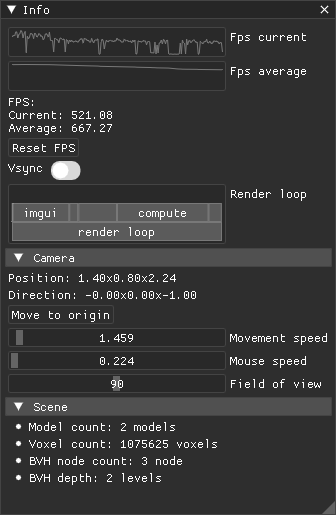
\includegraphics[scale=1]{images/dp_ui_info.png}
        	\caption{\textbf{Informační okno}}
        	\label{fig:info_ui}
	\end{subfigure}\\
	\caption{Ukázka oken demonstrační aplikace}
	\label{fig:UI}
\end{figure}


UI aplikace je rozděleno do následujících částí:

\begin{itemize}
	\item Info - zobrazení statistik vykreslování (počet snímků za sekundu, flame graph), informace o~kameře a její parametry, a také informace o právě vykreslované scéně.
	\item Render settings - výběr typu zobrazení (stínování, normály, počet iterací, hloubka v~stromě...), ovládání světla.
	\item Debug - memo pro výstup logů, připravený Chaiscript pro přidávání složitějších funkcí.
	\item Debug images - okno pro zobrazení textury reprezentující počet iterací při průchodu octree.
	\item Shader controls - ovládání parametrů pro shadery.
	\item Probe grid controls - ovládání mřížky sond.
	\item Models - ovládání modelů zobrazených ve scéně.
	\item Probes info - vizualizace atlasu sond a renderování scény pomocí něj.
\end{itemize}

\subsubsection{Konfigurace}
Důležitou součástí aplikace je konfigurační soubor, který je blíže popsán v příloze \ref{appendix:configfile}. Tento soubor obsahuje primárně informace o cestách ke zdrojům (cesta k modelům, shaderům...). Také je v něm obsažena definice velikosti okna demonstrační aplikace a velikost pracovní skupiny pro vykreslování za pomocí octree. Aplikace automaticky ukládá data, která uživatel nastavil v uživatelském rozhraní.

Typ souboru zvolený pro konfiguraci je \texttt{TOML}. Tento formát byl zvolen primárně z toho důvodu, že je velice snadno čitelný pro uživatele a není tedy nutné vytvářet separátní program pro manipulaci s konfigurací. Samozřejmě existují podobné, uživatelsky přívětivé, formáty, jako například \texttt{YAML} nebo \texttt{INI}, ale \texttt{TOML} byl zvolen také kvůli knihovně \texttt{toml++}, díky které je manipulace s konfiguračním souborem relativně pohodlná. 


\chapter{Vyhodnocení}
\label{testovani}
V~této kapitole je krátký popis dosažených výsledků týkající se doby převodu vstupních dat a také analýza využití paměti na grafické kartě.

\section{Převod vstupních dat na octree}
Převod vstupních dat na octree byl popsán v~sekci \ref{sec:voxel_conversion}. Převod je prozatím prováděn sekvenčně na jednom vlákně, ale v~budoucí verzi jej plánuji předělat tak, aby využíval více vláken procesoru. Na obrázku \ref{fig:time_convert} je graf závislosti času převodu na počtu vstupních voxelů. Graf \ref{fig:time_convert_mini} zobrazuje stejné měření s~aktivovanou minimalizací. Měření byla prováděna s~nejvyšší úrovní optimalizací kompilace. Pro měření bylo použito CPU \texttt{Ryzen 3600} a probíhalo na jednom vláknu za využití knihovny \texttt{nanobench}\footnote{\url{https://github.com/martinus/nanobench}}. Model, který byl v~testech použit byly plné koule o~různých poloměrech.


\begin{figure}[H]
	\begin{subfigure}{.5\textwidth}
		\begin{tikzpicture}[scale=0.7, transform shape]
			\begin{axis}[
				xlabel={velikost scény [voxely]},
				y unit = s,
				ylabel={doba zpracování},
				grid=both
				]
				\addplot table [x=size, y=time, mark=none, color=red]{data/time_convert.txt};
			\end{axis}
		\end{tikzpicture}
		\caption{Bez minimalizace}
		\label{fig:time_convert}
	\end{subfigure}
	\begin{subfigure}{.5\textwidth}
		\begin{tikzpicture}[scale=0.7, transform shape]
			\begin{axis}[
				xlabel={velikost scény [voxely]},
				y unit = s,
				ylabel={doba zpracování},
				grid=both
				]
				\addplot table [x=size, y=time, mark=none, color=red]{data/time_convert_mini.txt};
			\end{axis}
		\end{tikzpicture}
		\caption{S~minimalizací}
		\label{fig:time_convert_mini}
	\end{subfigure}
	\caption{Čas tvorby octree}
\end{figure}

I~když to není z~grafu moc znatelné, transformace s~minimalizací je o~pár procent rychlejší, jelikož není nutné vytvářet tak velký finální strom. Pokud by vstupní data byla pro minimalizaci nepříznivá, byla by tato metoda pomalejší.

Vzhledem k~rychlostem zpracování je jasné, že algoritmy nejsou příliš dobře optimalizované a mám v~úmyslu je v~budoucnu zrychlit.

\section{Paměťová náročnost}
V této sekci je popsána paměťová náročnost dvou hlavních částí částí programu. Jedná se o vyhodnocení využití VRAM.

\subsubsection{Octree}

Každý uzel octree zabírá v~prvé řadě 4 bajty (15 bitů \texttt{child pointer} + 1 bit \texttt{far} + 8 bitů \texttt{valid mask} + 8bitů \texttt{leaf mask}). Dále pro dohledání materiálů a ostatních parametrů další 4 bajty (24 bitů \texttt{value pointer} + 8 bitů \texttt{mask}). Tyto dva záznamy nejsou vytvářeny pro listové uzly. Pokud budeme předpokládat strom, který má prostor obsazený přesně z~50 \% a je obsazen pouze každý druhý voxel, s~hloubkou stromu 6 -- tedy 37448 voxelů -- celková obsazená paměť zmíněnými záznamy bude 18724 bajtů. Při popsaném rozložení voxelů se samozřejmě jedná o~nejhorší možný případ.

\begin{table}[H]
	\centering
	\begin{tabular}{|r|r|}
		\hline
		\multicolumn{1}{|c|}{hloubka stromu} & \multicolumn{1}{c|}{obsazená paměť {[}B{]}} \\ \hline
		1                                    & 4                                           \\ \hline
		2                                    & 36                                          \\ \hline
		3                                    & 292                                         \\ \hline
		4                                    & 2340                                        \\ \hline
		5                                    & 18724                                       \\ \hline
		6                                    & 149796                                      \\ \hline
	\end{tabular}
	\caption{Využití paměti podle hloubky stromu při maximální nepříznivosti podmínek}
\end{table}

Tímto jsou pokryta základní data popisující strom a vyhledávací strukturu do parametrů. Další paměť je využita \texttt{far} pointery. V~pesimistickém případě je může potřebovat \textasciitilde5 \% uzlů, ovšem jsou potřeba až pro hloubku stromu vyšší než 7, kvůli množství potomků v~úrovni.

Poslední data vyžadující velké množství paměti jsou samotné parametry voxelů. Samozřejmě záleží na využitých parametrech, pro phongovo stínování je dostačující barva, tedy 4 bajty (RGBA formát, kde je každý kanál reprezentován 8 bity). Samozřejmě se data dají zakódovat efektivněji.

Celková paměťová náročnost pro octree se zmíněnými parametry je tedy:

\begin{table}[H]
	\centering
	\begin{tabular}{|r|r|}
		\hline
		\multicolumn{1}{|c|}{hloubka stromu} & \multicolumn{1}{c|}{využití paměti {[}B{]}} \\ \hline
		1                                    & 20                                          \\ \hline
		2                                    & 164                                         \\ \hline
		3                                    & 1316                                        \\ \hline
		4                                    & 10532                                       \\ \hline
		5                                    & 84260                                       \\ \hline
		6                                    & 674084                                      \\ \hline
	\end{tabular}
\end{table}

Ve všech případech se jedná o~nejhorší možný případ. Realisticky použitelné modely mají paměťovou náročnost výrazně nižší a také u~nich dochází k~minimalizaci stromu (která v~uvažovaném nejhorším případě není možná).


\subsubsection{Light field probes}
Jak bylo zmíněno v sekci \ref{sec:lfp_design}, každá sonda sestává ze dvou textur, první z nich má rozlišení 1024x1024 s datovým typem \texttt{RG32F}, tedy využívá 8 bajtů paměti. Z těchto 8 bajtů jsou 4 využity pro radianci/nepřímé osvětlení, 2 pro normály a 2 pro hloubku. Druhá textura má $\frac{1}{16}$ rozlišení hlavní textury a obsahuje pouze informace o hloubce. Datovým typem této textury je \texttt{R16F}, což znamená, že každý texel zabírá 2 bajty. Využití paměti jedné sondy je tedy 8396800 bajtů (\textasciitilde{}8.4 MB).

Samozřejmě není použita jen jedna sonda. Množství sond je, kvůli implementaci algoritmů s nimi pracujících, omezeno na mocniny dvou v každé ose. V následující tabulce je seznam využití paměti pro množství sond, které se nejpravděpodobněji využijí.

\begin{table}[H]
	\centering
\begin{tabular}{|l|l|}
\hline
počet sond & využití paměti {[}MB{]} \\ \hline
1          & 8.4                     \\ \hline
4          & 33.5                    \\ \hline
16         & 134.3                   \\ \hline
128        & 1074.8                  \\ \hline
512        & 4299.1                  \\ \hline
\end{tabular}
\end{table}


\section{Výsledky}

\chapter{Závěr}
\label{zaver}
Cílem semestrální části diplomové práce bylo nastudovat techniky fotorealistického zobrazování voxelových modelů a nástrojů, pomocí nichž toho lze dosáhnout a také vytvořit kostru aplikace. Demonstrační aplikace je schopna načítat a transformovat modely a také zobrazovat voxelové scény.

V~teoretické části dokumentu byl popsán princip realistického zobrazování a některé metody pro dosažení realistického výsledku. Byl popsán například algoritmus ray tracing s~některými jeho obměnami. Sekce také představila základy práce s~materiály a metody pro odstranění aliasingu. Další sekce vysvětlila princip voxelizace prostoru a představila některá jeho využití. Také zde byly popsány metody pro vykreslení voxelů a základní hierarchické struktury, pomocí nichž lze zmíněné vykreslování akcelerovat.

Kapitola návrhu řešení popsala způsob efektivní reprezentace voxelových dat a vysvětlila její výhody. V~této kapitole je taky popsán návrh vykreslování voxelových scén.

Implementační část obsahovala výčet použitých nástrojů a knihoven. Ve zkratce také předvedla knihovny, které byly v~rámci tvorby projektu vytvořeny. Tyto knihovny jsou na projektu plně nezávislé a lze je použít pro libovolnou další tvorbu. V~kapitole byl také popsán algoritmus pro vytvoření octree z~voxelových dat a jeho minimalizace. V~poslední sekci bylo krátce popsáno uživatelské rozhraní demonstrační aplikace.

Poslední kapitola, vyhodnocení, se zabývala časovou náročností tvorby a minimalizace octree a paměťové náročnosti této struktury. Algoritmus tvorby octree má velké rezervy a mám v~úmyslu ho do budoucna optimalizovat. Paměťová náročnost octree struktury je ale poměrně nízká, z~ohledem na to, kolik dat v~ní reprezentujeme. V~sekci byly uvedeny hodnoty nejhoršího případu.

Cíl další práce je jasný: implementovat alternativní způsob vykreslování (light field probes \ref{sec:light_field_probes}) a umožnit vykreslování výrazně větších scén. Také optimalizovat načítání scén pro použití v~reálném čase a navrhnout způsob reprezentace velkých scén a jejich dynamické načítání z~disku.


%===============================================================================
